\documentclass[landscape]{foils} 
%\newif\ifpdf
%\ifx\pdfoutput\undefined
%\pdffalse % we are not running PDFLaTeX
%\else
%\pdfoutput=1 % we are running PDFLaTeX
%\pdftrue
%\fi

%\ifpdf
\usepackage[pdftex]{graphicx}
%\else
%\usepackage{graphicx}
%\fi

%\ifpdf
\DeclareGraphicsExtensions{.pdf, .jpg, .tif, .png}
%\else
%\DeclareGraphicsExtensions{.eps, .jpg}
%\fi

%\usepackage{pslatex}
\usepackage{tabularx,dcolumn, graphicx, amsfonts,amsmath}  
\usepackage[sectionbib]{natbib}
\bibliographystyle{apalike}
\usepackage{picinpar}
\usepackage{multirow}
\usepackage{rotating}
\usepackage{paralist} %compactenum
\setlength{\voffset}{-0.5in}
%\setlength{\hoffset}{-0.5in}
%\setlength{\textwidth}{10.5in}
\setlength{\textheight}{7in}
\setlength{\parindent}{0pt}
%\pagestyle{empty}
%\renewcommand{\baselinestretch}{2.0}
\DeclareMathSymbol{\expect}{\mathalpha}{AMSb}{'105}
\def\p{\rm p}
\def\pp{\rm P}
% this are commands that come with the color package
\usepackage{color}
\usepackage{fancyhdr}


\pagestyle{empty}
%define colors
\definecolor{mediumblue}{rgb}{0.0509,0.35,0.568}
\definecolor{blue}{rgb}{0.0109,0.15,0.468}
\definecolor{black}{rgb}{0.04,0.06,0.2}
\definecolor{darkblue}{rgb}{0.03,0.1,0.2}
\definecolor{darkgreen}{rgb}{0.03,0.5,0.2}
\definecolor{lightblue}{rgb}{0.85,0.9333,0.95}
\definecolor{lightblue2}{rgb}{0.270588, 0.45098, 0.701961}
\definecolor{white}{rgb}{1.0,1.0,1.0}
\definecolor{yellow}{rgb}{0.961,0.972,0.047}
\definecolor{red}{rgb}{0.9,0.1,0.1}
\definecolor{orange}{rgb}{1.0,0.4,0.0}
\definecolor{grey}{rgb}{0.5,0.5,0.5}
\definecolor{violet}{rgb}{0.619608, 0.286275, 0.631373}
\definecolor{mybackgroundcolor}{rgb}{1.0,1.0,1.0}

%\definecolor{light}{rgb}{.5,0.5,0.0}
\definecolor{light}{rgb}{.3,0.3,0.3}

% sets backgroundcolor for whole document 
\pagecolor{mybackgroundcolor}
% sets text color
%\color{black}
% see below for an example how to change just a few words
% using \textcolor{color}{text}

\font \courier=pcrb scaled 2000
\newcommand{\notetoself}[1]{{\textsf{\textsc{\color{red} #1}}}\\}

\newcommand{\answer}[1]{{\sf \color{red} #1}}

\usepackage{pdfpages}

\newcommand{\section}{\secdef \newsection\newsection}
%\renewcommand{\labelitemi}{\includegraphics[width=5mm]{images/bullet.pdf}}
\newcommand{\newsection}[1]{%
{
	\par\flushleft\large\sf\bfseries \vskip -2cm #1\\\rule[0.7\baselineskip]{\textwidth}{0.5mm}\par}}

\newcommand{\subsection}{\secdef \test\test}
\newcommand{\test}[1]{%
	{\par\flushleft\normalsize\sf\bfseries #1: }}
\newcommand{\M}{\mathcal{M}}
\newcommand{\prob}{{\rm Prob~}}
\def\showy#1{{\normalsize\sf\bfseries #1}}
\def\donotuse#1{}

\newcommand{\entrylabel}[1]{\mbox{#1}\hfil}
\newenvironment{entry}
	{\begin{list}{}%
		{\renewcommand{\makelabel}{\entrylabel}%
		\setlength{\labelwidth}{35pt}%
		\setlength{\leftmargin}{\labelwidth+\labelsep}%
	}%
	{\end{list}}}

\newcommand{\poltext}{{\copyright\ 2002--2010 by Paul O. Lewis -- Modified by  Mark Holder with permission from Paul Lewis}}

\newcommand{\pol}{{\footnotesize \poltext}}
\newcommand{\myBackground}{\begin{picture}(0,0)(0,0)  \put(-40,-70){\makebox(0,0)[l]{\includegraphics[width=33cm]{images/baby_blue.jpg}}} \end{picture}}
\newcommand{\myFooter}{}
%\begin{picture}(0,0)(0,0)
%	\put(0,-185){\pol}
%\end{picture}}
\newcommand{\myNewSlide}{\newpage\myFooter} % \myBackground}

\usepackage{url}
\usepackage{hyperref}
\hypersetup{backref,  linkcolor=blue, citecolor=red, colorlinks=true, hyperindex=true}

\begin{document}
\pagecolor{white}
\unitlength=1mm
\begin{center}
{\Large Many of the  slides that I'll use have been borrowed from Dr.\ Paul Lewis, Dr.\ Joe Felsenstein. Thanks!}
\vskip 15mm
\large Paul has many great tools for teaching phylogenetics at his web site: \\
\url{http://hydrodictyon.eeb.uconn.edu/people/plewis}
\end{center}

\myNewSlide
\myNewSlide
\section*{The main subject of this course: estimating a tree from character data}
Tree construction:
\begin{compactitem}
	\item strictly algorithmic approaches - use a ``recipe'' to construct a tree
	\item optimality based approaches - choose a way to ``score'' a trees and then search for the tree that has the best score.
\end{compactitem}
Expressing support for aspects of the tree:
\begin{compactitem}
	\item bootstrapping,
	\item testing competing trees against each other,
	\item posterior probabilities (in Bayesian approaches).
\end{compactitem}


\myNewSlide
Simple test of Bergmann's rule: comparing latitude and mass (I made these data up)\\
\normalsize
lat. offset = degrees north of the 49th parallel.
\begin{table}[htdp]
\begin{center}
\begin{tabular}{|c|c|c|}
\hline
species & lat. offset & mass \\
\hline
L1 &  3.1 &  5.9 \\
L2 &  5.4  & 4.3 \\
L3 &  5.1 &  3.1 \\
L4 &  1.8 &  3.6 \\
H1 &  13.5  & 15.2 \\
H2 &  14.6 &  13.5 \\
H3 &  13.6 &  12.4 \\
H4 &  10.8 &  13.7 \\
\hline

\end{tabular}
\end{center}
\label{default}
\end{table}%
\myNewSlide
\begin{picture}(0,0)(0,0)
	\put(-50,-185){\makebox(0,0)[l]{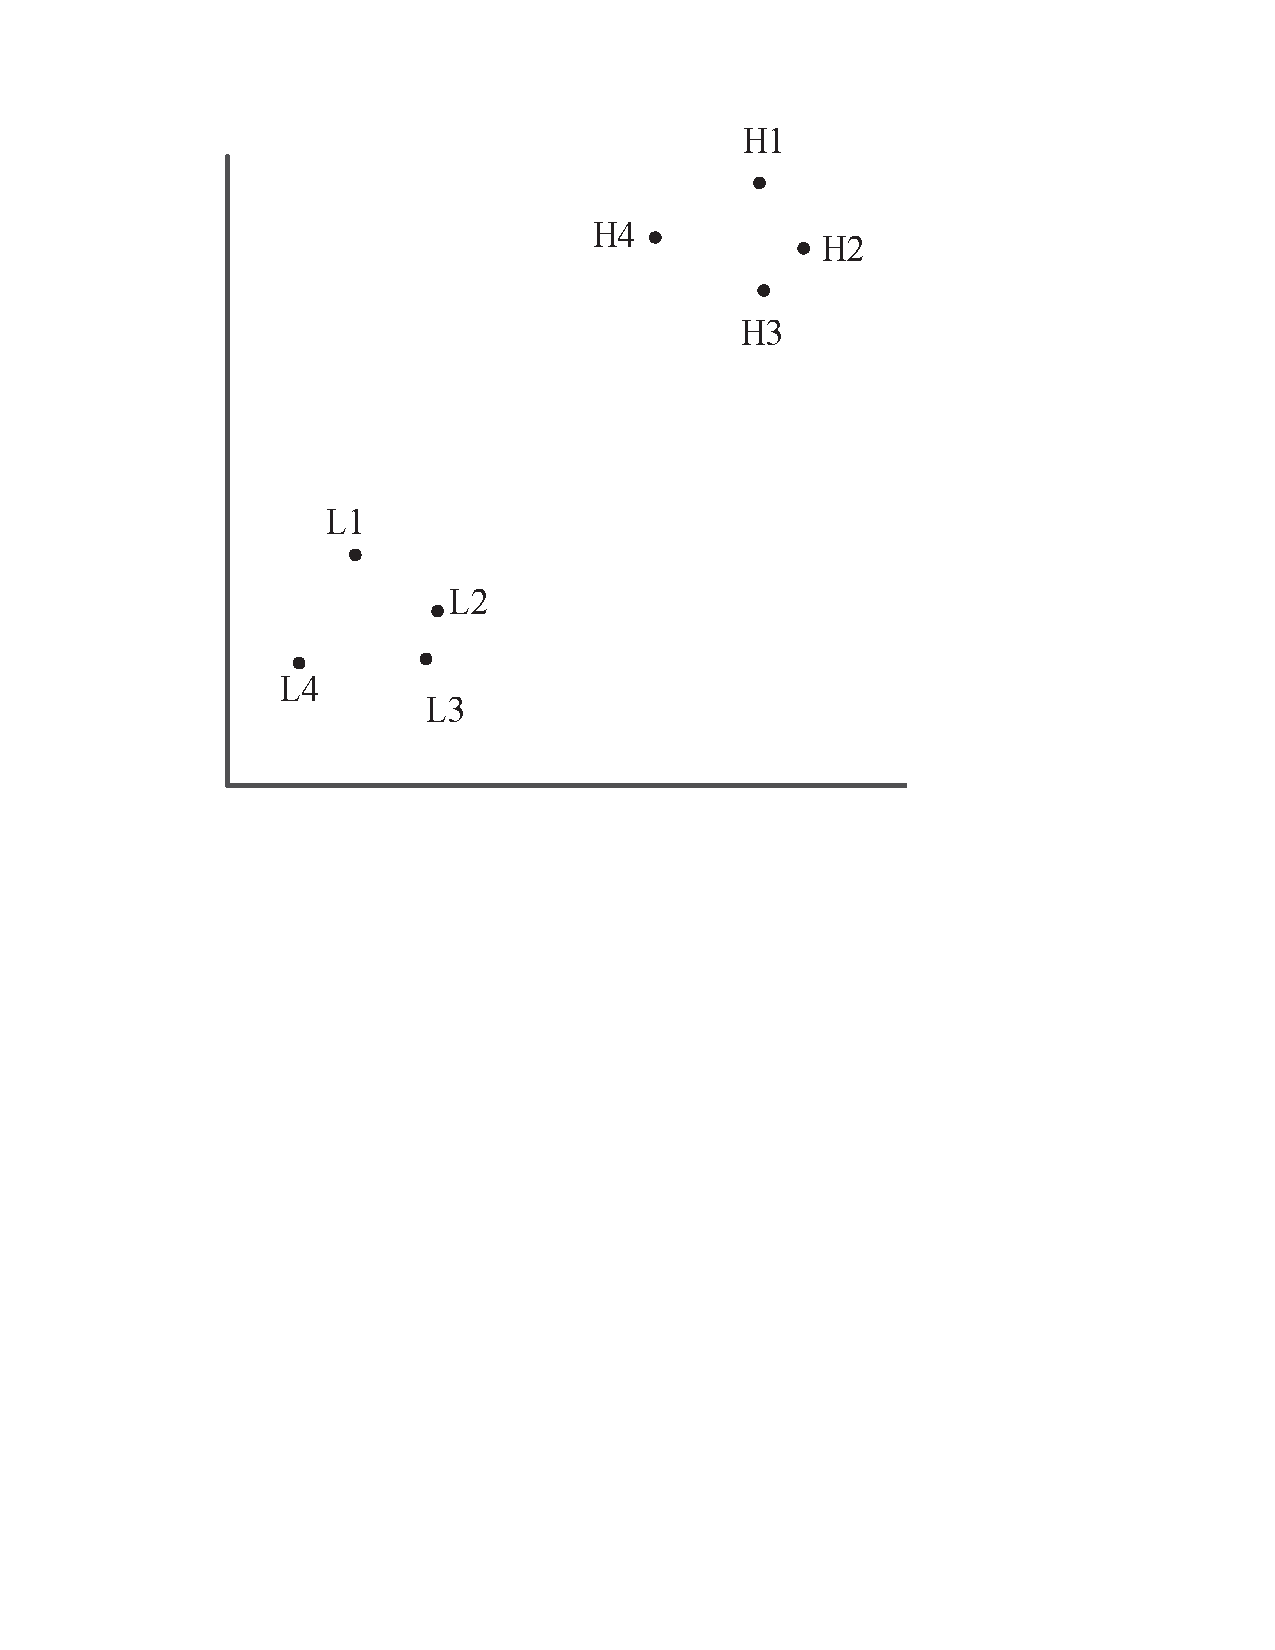
\includegraphics[scale=1.5]{../images/pattern.pdf}}}
\end{picture}

\myNewSlide
(cue cartoon videos)

See \url{http://phylo.bio.ku.edu/slides/no-correl-anim.mov}

and \url{http://phylo.bio.ku.edu/slides/correl-anim2.mov}

\myNewSlide
\section*{No (or little) evidence for correlation}
\begin{picture}(0,0)(0,0)
	\put(-20,-145){\makebox(0,0)[l]{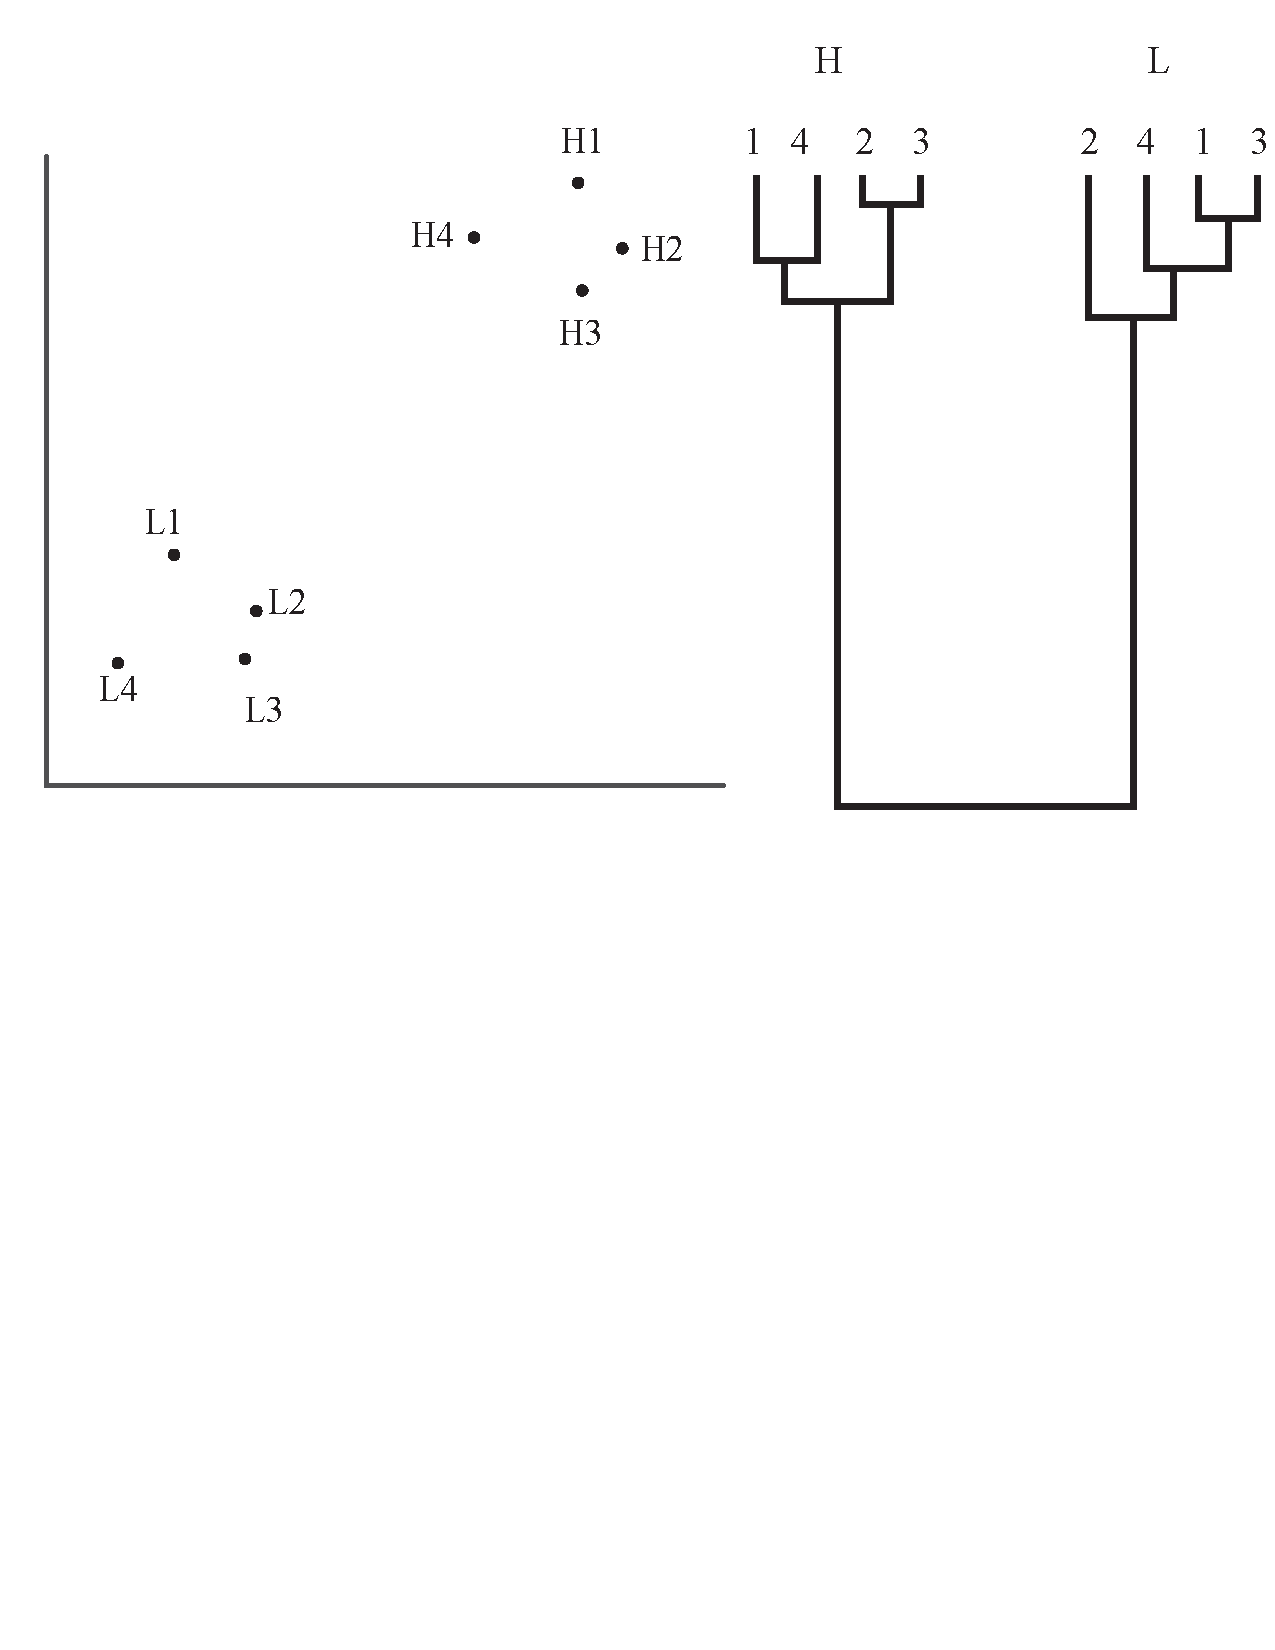
\includegraphics[scale=1.2]{../images/pattern-no-correl.pdf}}}
\end{picture}

\myNewSlide
\section*{Evidence for correlation}
\begin{picture}(0,0)(0,0)
	\put(-20,-145){\makebox(0,0)[l]{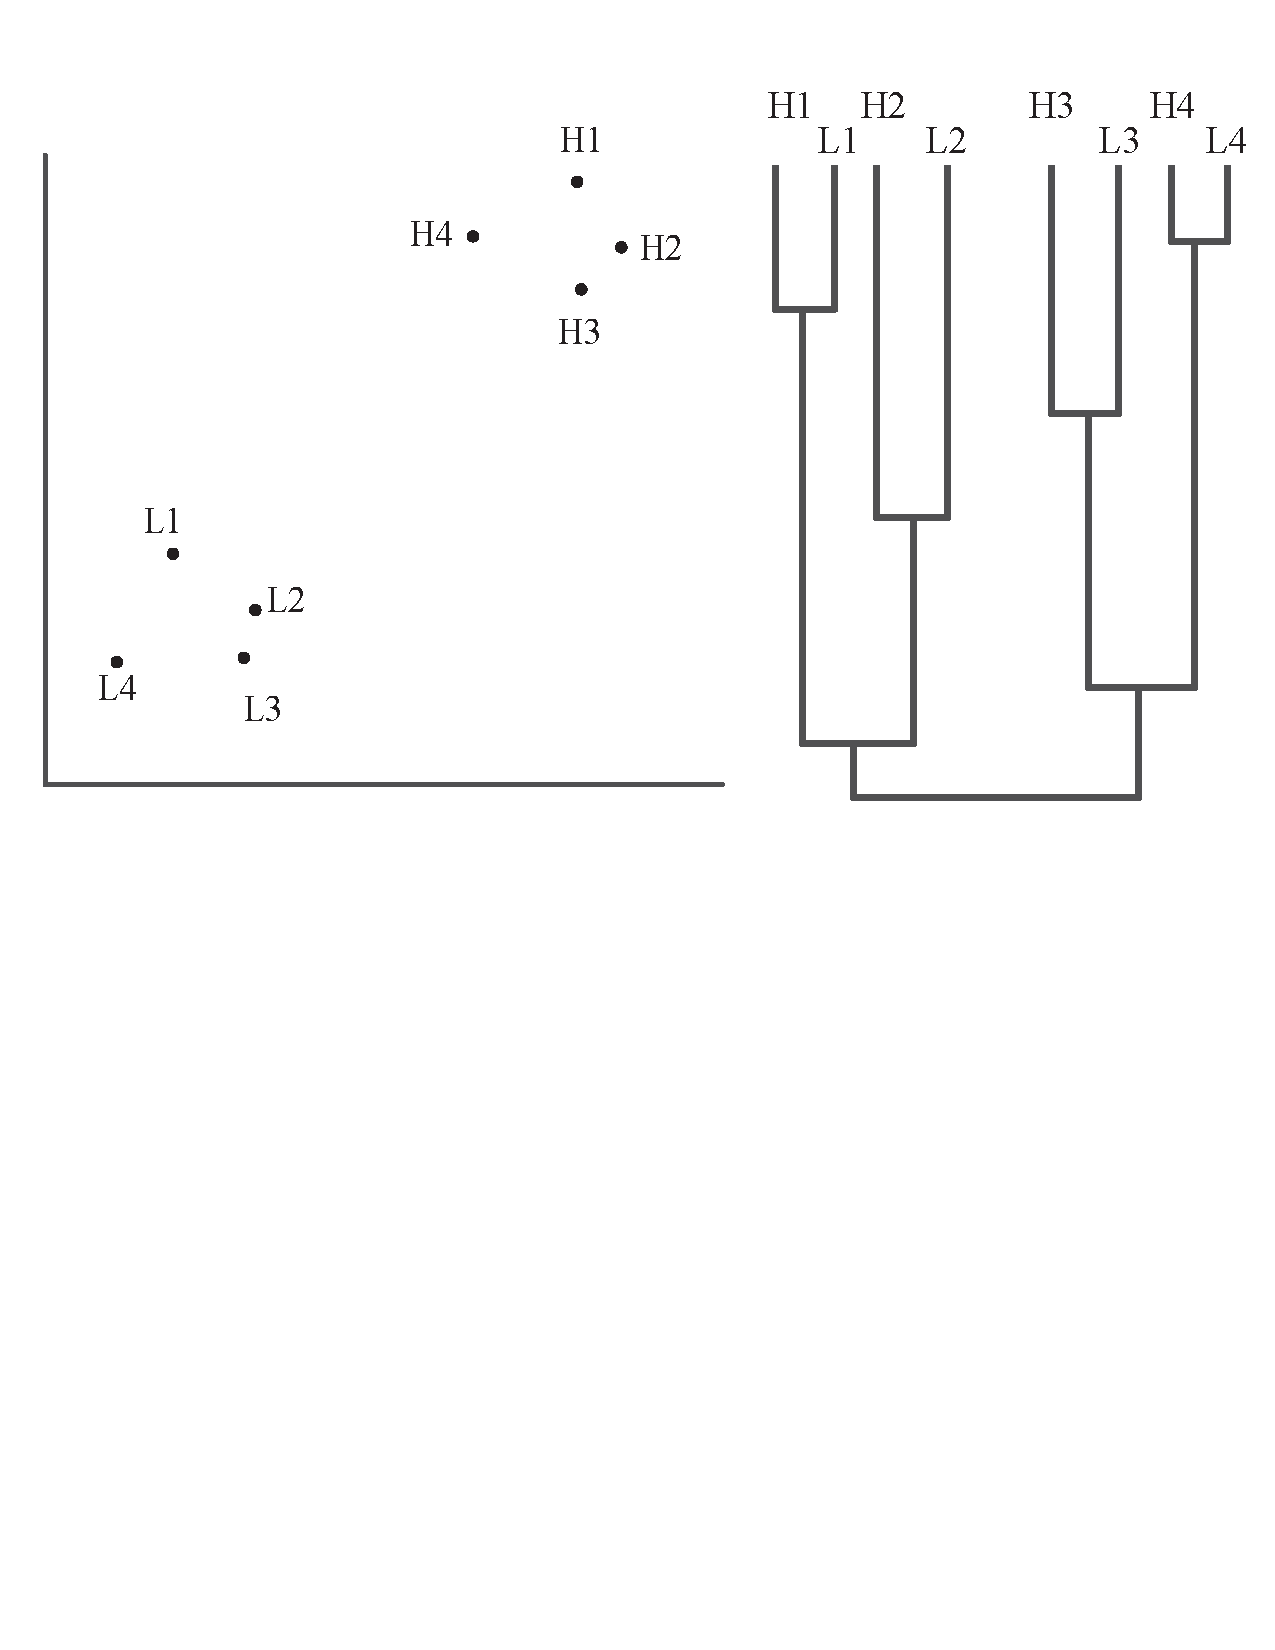
\includegraphics[scale=1.2]{../images/pattern-correl.pdf}}}
\end{picture}

\myNewSlide
\section*{Do desert green algae use xanthophyll to protect against excessive light intensities?}
\begin{center}
\begin{tabular}{|c|c|c|}
	\hline
	Species \hskip 2mm & Habitat \hskip 4mm & Photoprotection\\
	\hline 1 & terrestrial & xanthophyll \\
	\hline 2 & terrestrial & xanthophyll \\
	\hline 3 & terrestrial & xanthophyll \\
	\hline 4 & terrestrial & xanthophyll \\
	\hline 5 & terrestrial & xanthophyll \\
	\hline 6 & aquatic & none \\
	\hline  7 & aquatic & none \\
	\hline 8 & aquatic & none \\
	\hline  9 & aquatic & none \\
	\hline 10 & aquatic & none \\
	\hline
\end{tabular}
\end{center}

\myNewSlide
\section*{Phylogeny reveals the events that generate the pattern}
\begin{picture}(0,0)(0,0)  \put(-15,-65){\makebox(0,0)[l]{\includegraphics[scale=1.2]{../nonfreeimages/pol/char_correlation.pdf}}}
\put(-25,-140){1 pair of changes.}
\put(-25,-150){Coincidence?}
\put(110,-140){5 pairs of changes.}
\put(110,-150){Much more convincing}
\end{picture}

\myNewSlide
\section*{Inferring Process from Pattern}
{\large
Hypothesis:\par
	Gregariousness should arise more frequently in unpalatable organisms than in tasty ones \citep{SillenT1988}
}

\myNewSlide
\section*{Inferring Process from Pattern}
\begin{picture}(-0,0)(-0,0)
	\put(0,0){\makebox(30,-150)[l]{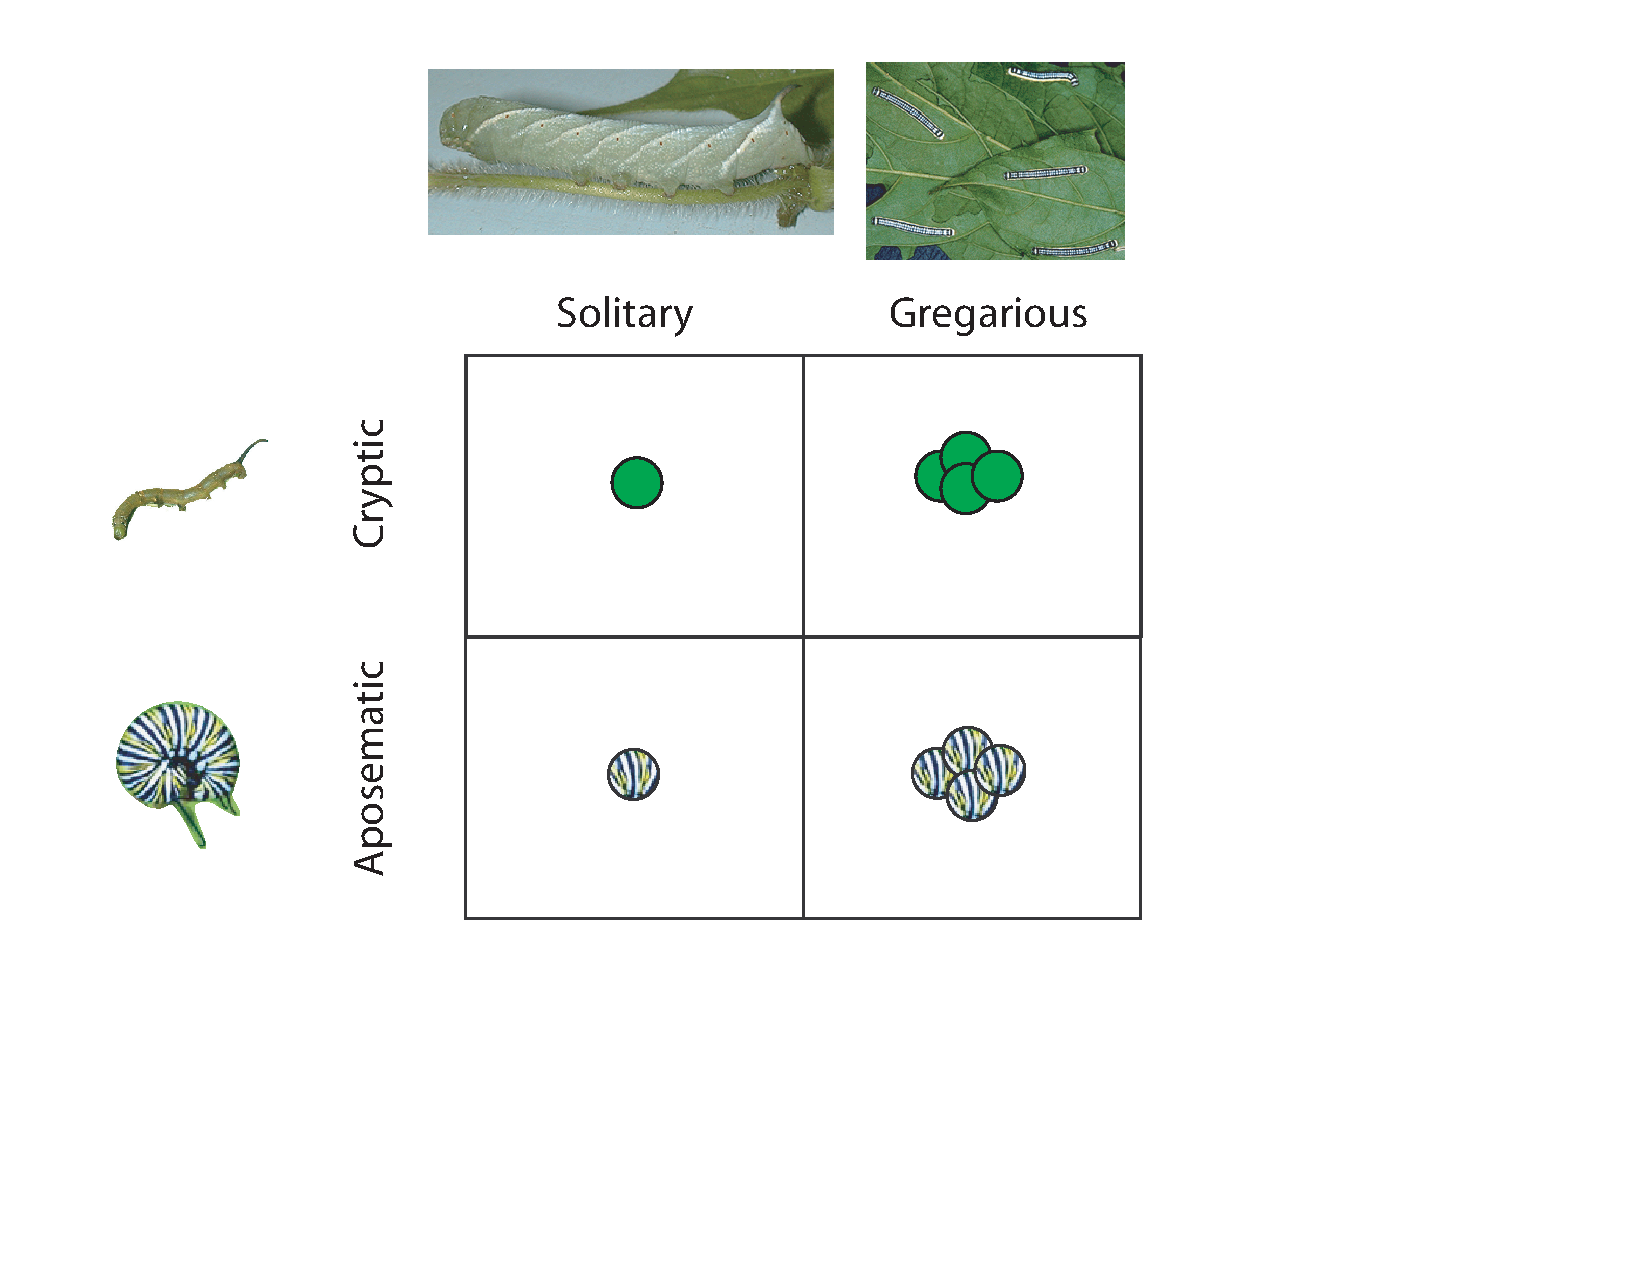
\includegraphics[scale=1.]{../images/cat_legend.pdf}}}
	\put(25,-145){\small \citet{SillenT1988}, \citet{Dyer2002}, \citet{Hill2001}}
\end{picture}


%\myNewSlide
%\section*{Inferring Process from Pattern}
%Some (fake) data:\\
%\begin{picture}(-0,0)(-0,0)
%	\put(-50,-150){\makebox(10,-150)[l]{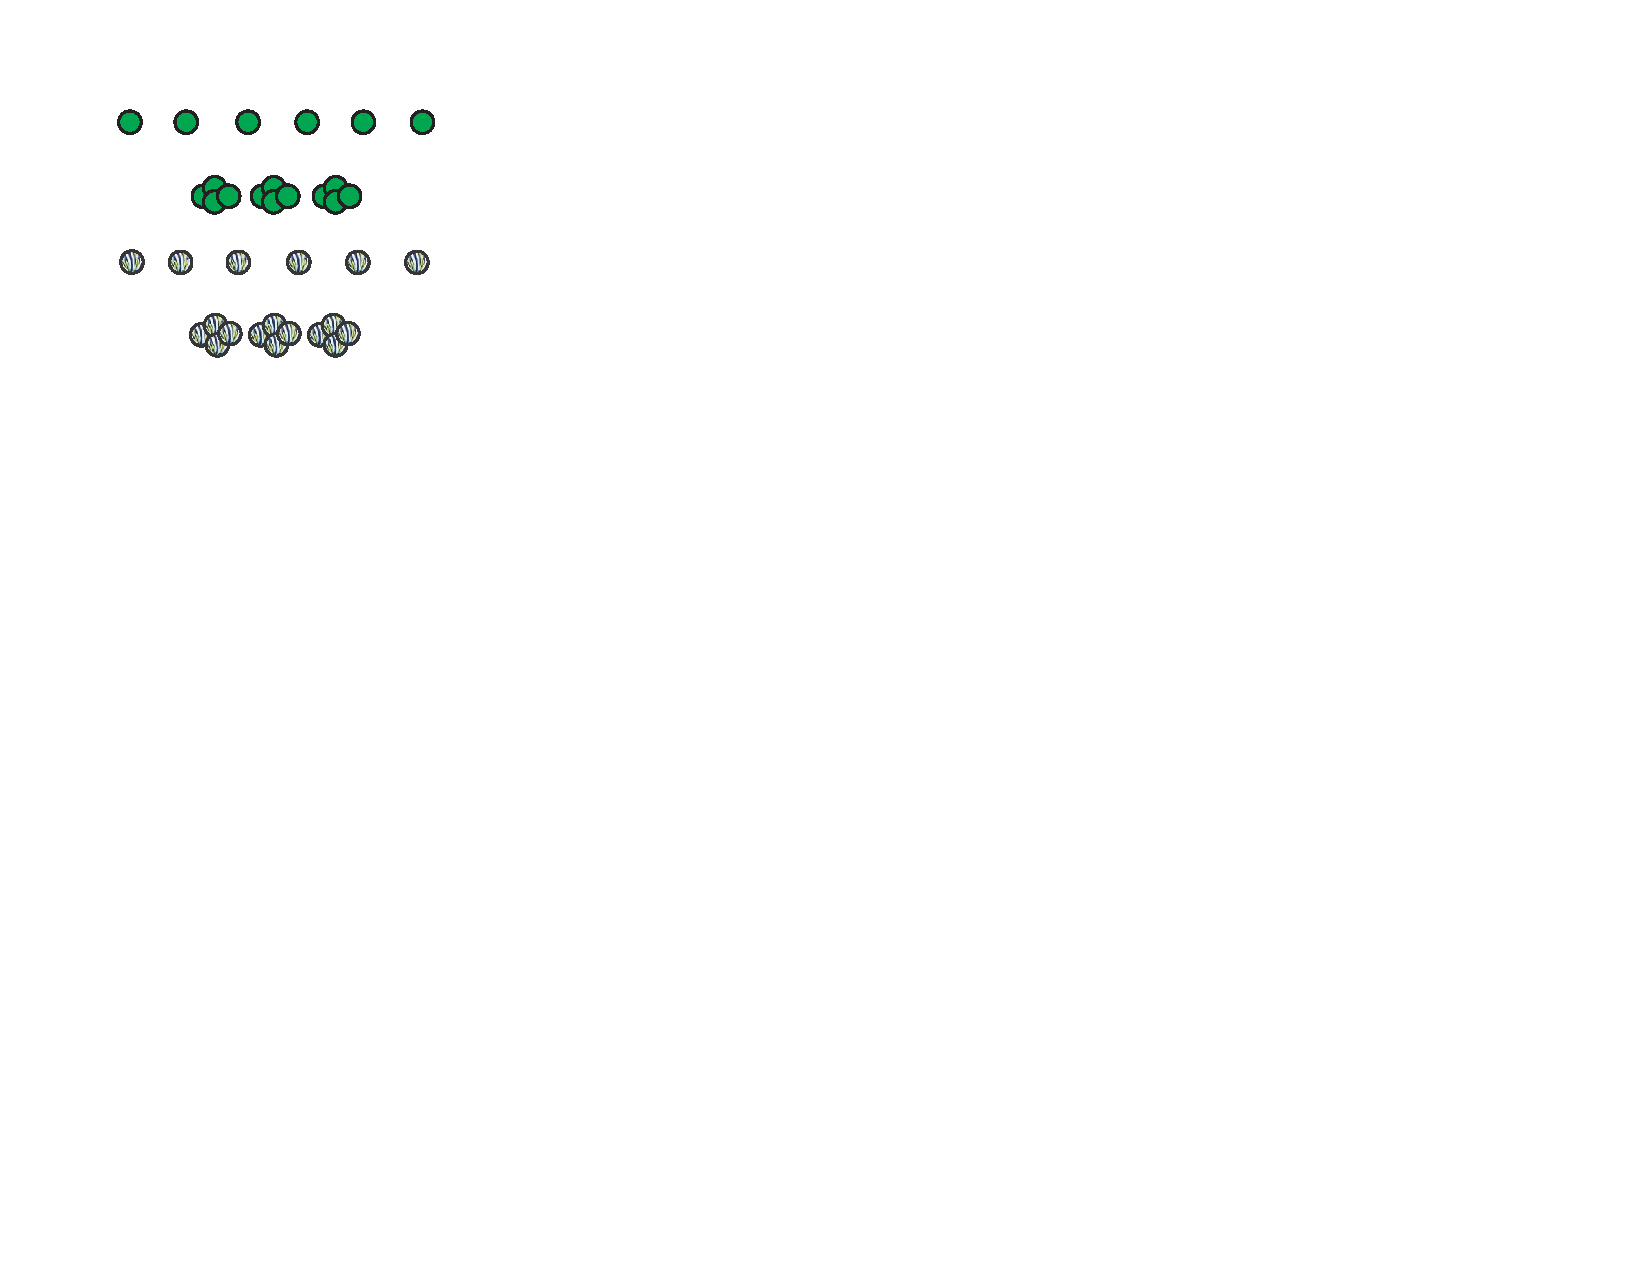
\includegraphics[scale=2.4]{../images/nonPhylogeneticData.pdf}}}
%	\put(130,-18){6 cryptic, solitary species}
%	\put(130,-47){3 cryptic, gregarious species}
%	\put(130,-75){6 aposematic, solitary species}
%	\put(130,-105){3 aposematic, gregarious species}
%\end{picture}

\myNewSlide
\begin{picture}(-0,0)(-0,0)
	\put(-10,-60){\makebox(30,-150)[l]{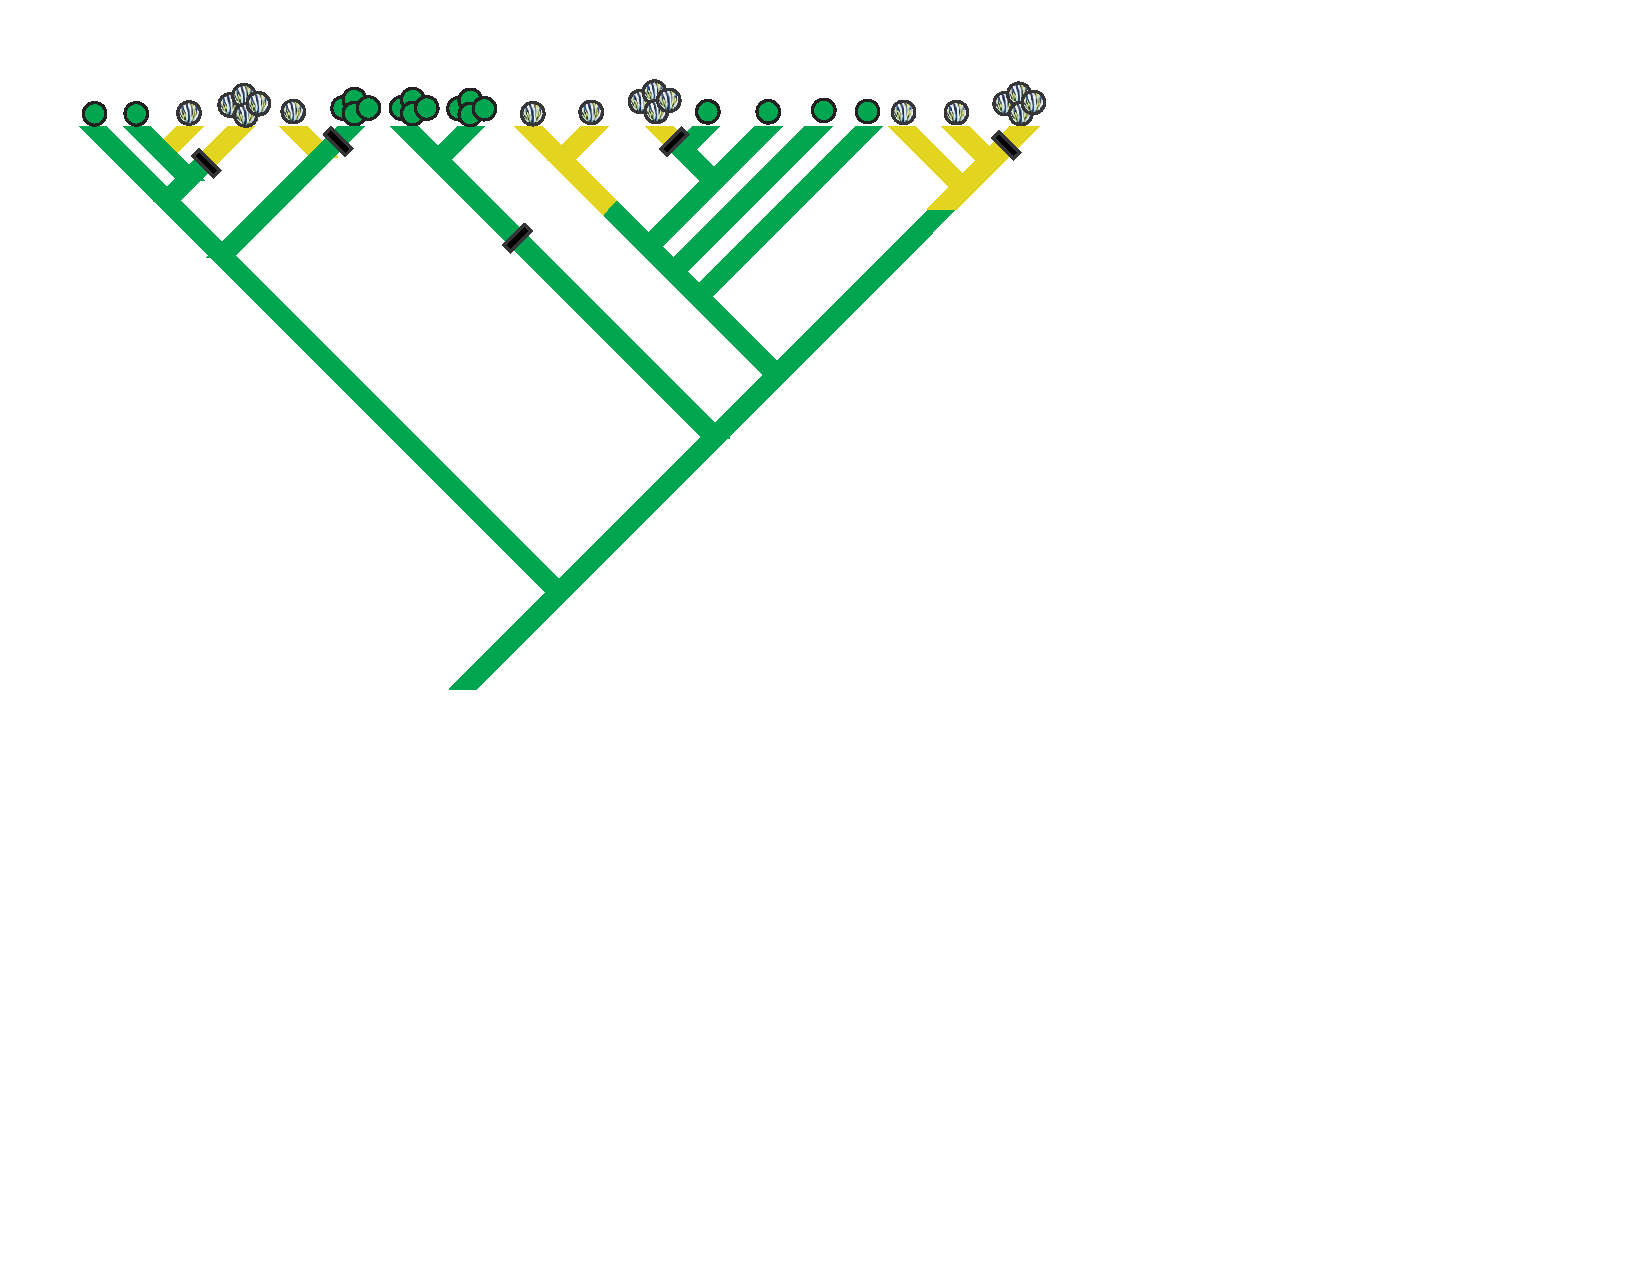
\includegraphics[scale=1.4]{../images/noassoc.pdf}}}
	\put(5,-170){One possible outcome:  }
	\put(10,-180){No clear evidence of associations between traits}
\end{picture}

\myNewSlide
\begin{picture}(-0,0)(-0,0)
	\put(-10,-60){\makebox(30,-150)[l]{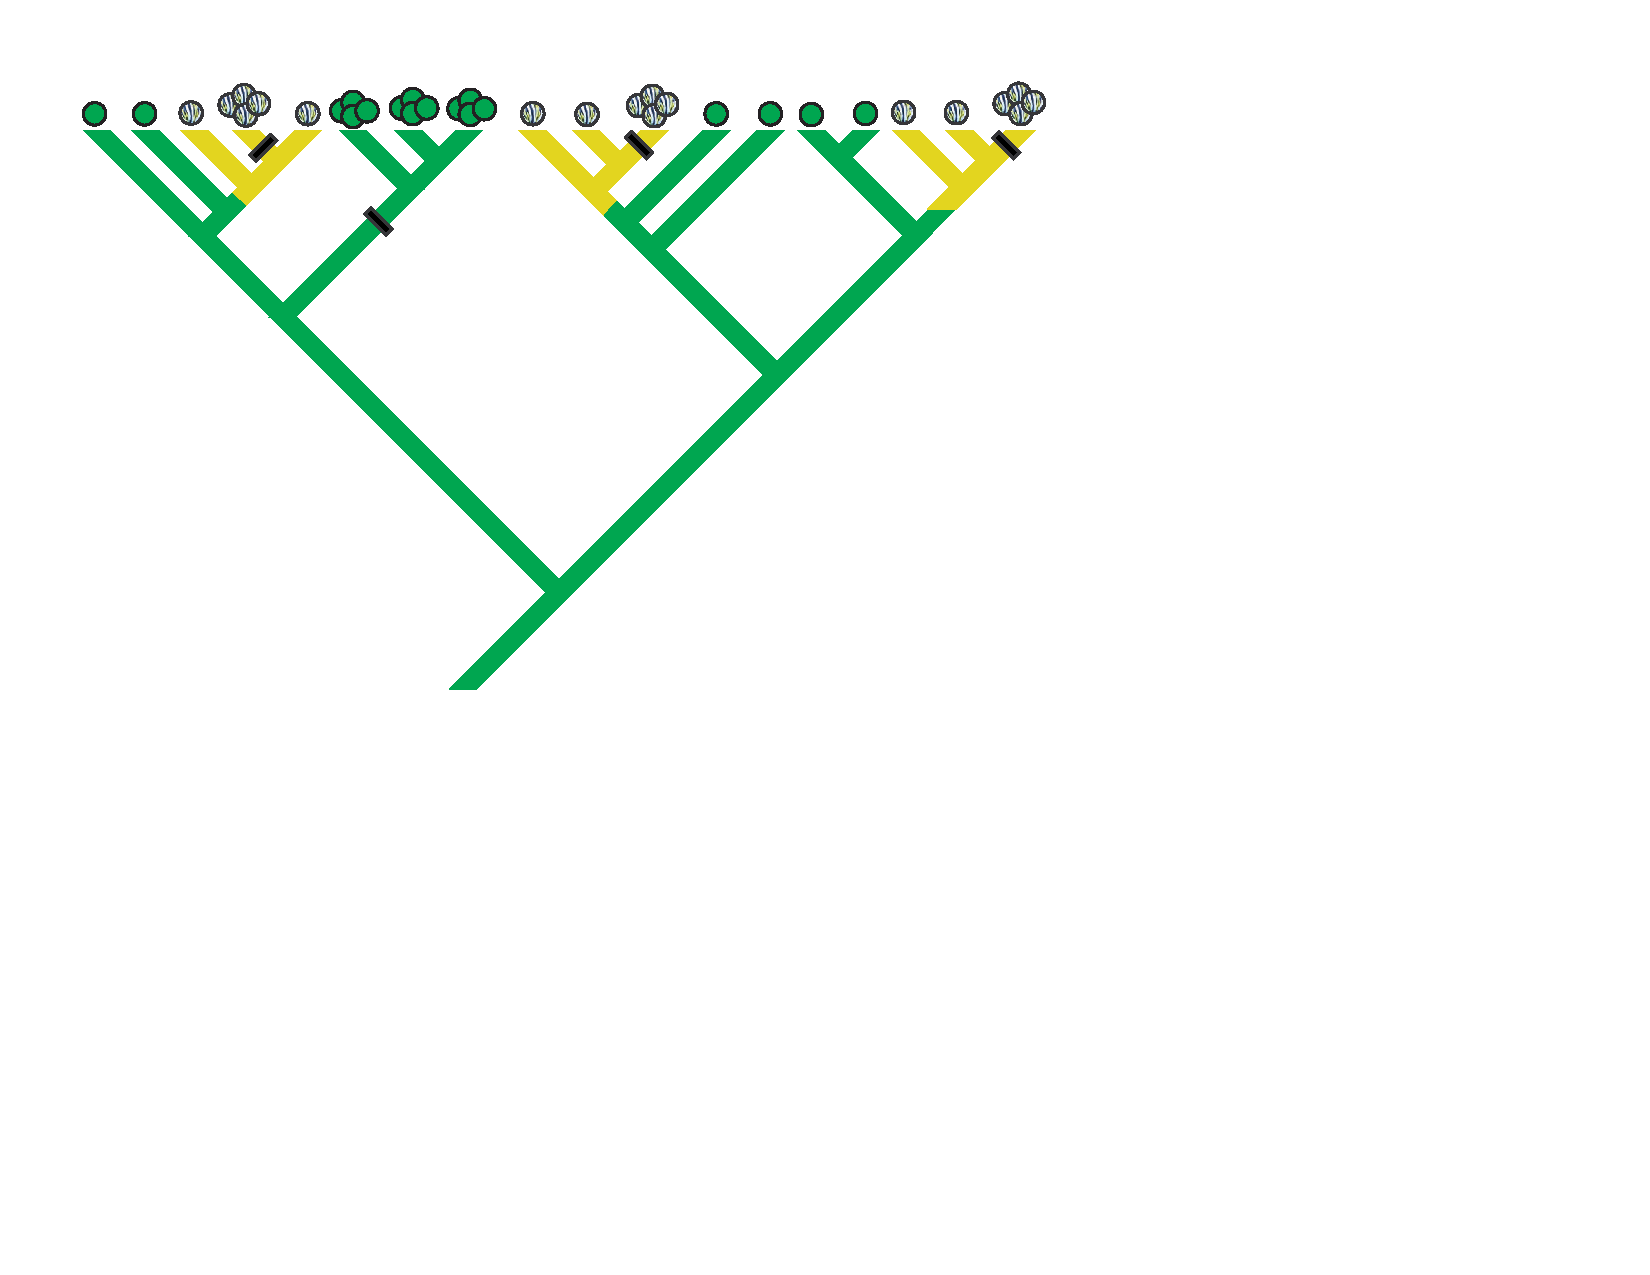
\includegraphics[scale=1.4]{../images/stTree.pdf}}}
	\put(5,-170){Cartoon of the real results \citep{SillenT1988}}
	\put(5,-180){Aposematic species are more likely to evolve gregarious larvae}
\end{picture}

\myNewSlide
\section*{Importance of phylogeny}
The previous slides had identical patterns of traits if the phylogeny is ignored.

Without knowledge of the tree, no conclusion would be reached.




\myNewSlide

\begin{picture}(0,0)(0,0)
	\put(-5,-85){\makebox(0,0)[l]{\includegraphics[scale=1.2]{../nonfreeimages/other/ButterflyMimicTree.jpg}}}
	\put(15,-165){\small Figure by Mathieu Joron: \url{http://xyala.cap.ed.ac.uk/joron/}}
\end{picture}

\myNewSlide

\begin{picture}(0,0)(0,0)
	\put(-5,-65){\makebox(0,0)[l]{\includegraphics[scale=2]{../nonfreeimages/other//HivRambautPCH2004.pdf}}}
	\put(15,-165){Figure from Rambaut, Posada, Crandall, and Holmes} 	\put(35,-175){{\bf Nature Reviews Genetics}, 2004}
\end{picture}


\myNewSlide
\begin{picture}(0,0)(0,0)
	\put(25,-65){\makebox(0,0)[l]{\includegraphics[scale=1.5]{../nonfreeimages/other/HivForensics.pdf}}}
	\put(15,-165){Figure from \citet{MetzkerMLPGH2002}, 2004}
\end{picture}


\myNewSlide
\section*{Tree terminology}
\begin{picture}(0,0)(0,0)  \put(-15,-70){\makebox(0,0)[l]{\includegraphics[scale=1.]{../nonfreeimages/pol/tree_terms.pdf}}}
\end{picture}


\myNewSlide
\section*{Rooted tree terminology}
\begin{picture}(0,0)(0,0)  \put(-15,-70){\makebox(0,0)[l]{\includegraphics[scale=1.]{../images/rtree_terms.pdf}}}
\end{picture}


\myNewSlide
\section*{Rooted tree terminology}
\begin{picture}(0,0)(0,0)  \put(-15,-70){\makebox(0,0)[l]{\includegraphics[scale=1.]{../images/utree_terms.pdf}}}
\end{picture}

\myNewSlide
\section*{Tree terms}
A tree is a connected, acyclic graph.

A rooted tree is a connected, acyclic directed graph.

A polytomy or multifurcation is a node with a degree $>$ 3 (in an unrooted tree), or a node with an out-degree $>2$ (in a rooted tree).

Collapsing an edge means to merge the nodes at the end of the branch (resulting in a polytomy in most cases).

Refining a polytomy means to ``break'' the node into two nodes that are connected by an edge.





\myNewSlide
\section*{Monophyletic groups (``clades''): the basis of phylogenetic classification}
\begin{picture}(0,0)(0,0)  \put(-10,-60){\makebox(0,0)[l]{\includegraphics[scale=1.2]{../nonfreeimages/pol/monophyletic.pdf}}}
\end{picture}

\myNewSlide
\section*{Paraphyletic groups: error of omitting some species}
\begin{picture}(0,0)(0,0)
	\put(-10,-60){\makebox(0,0)[l]{\includegraphics[scale=1.2]{../images/paraphyletic.pdf}}}
\end{picture}

\myNewSlide
\section*{Polyphyletic groups: error of grouping ``unrelated'' species}
\begin{picture}(0,0)(0,0)
	\put(-10,-60){\makebox(0,0)[l]{\includegraphics[scale=1.2]{../images/polyphyletic.pdf}}}
\end{picture}


\myNewSlide
\section*{Homework \#1 -- (due Monday, Aug 28th)}
\normalsize
Draw an unrooted tree from the table of splits shown on the next page.
The frequencies shown in the table represent bootstrap proportions.
We'll cover bootstrapping later in the course -- for now you can treat
the ``Freq'' column as label for the branches.

Start at the first row and add splits until you cannot add any more
splits to the tree.

Make sure to label the leaves of the tree with the taxon number
and the edges with the value found in the ``Freq'' column.



\myNewSlide
\begin{center}
{\tt 
\begin{tabular}{|lp{0.1cm}r|}
\hline
000000000111111 & & \\
123456789012345 & & Freq \\
\hline
..........*.*.* & & 100 \\
........**..... & & 99 \\
.**..........*. & & 97 \\
........***.*.* & & 94 \\
......*....*... & & 78 \\
...**********.* & & 67 \\
.**............ & & 61 \\
......*.*****.* & & 60 \\
..........*...* & & 56 \\
...*.*......... & & 41 \\
..........*.*.. & & 39 \\
..*..........*. & & 37 \\
.....********.* & & 33 \\
\hline
\end{tabular}
}
\end{center}
/end-of-homework








\myNewSlide
\section*{Branch rotation does not matter}
\begin{picture}(0,0)(0,0) 
 \put(-15,-40){\makebox(0,0)[l]{\includegraphics[scale=1.]{../nonfreeimages/pol/rotate_tree.pdf}}}
 \large
 \put(0,-15){A}
 \put(21,-15){C}
 \put(42,-15){E}
 \put(63,-15){B}
 \put(84,-15){F}
 \put(105,-15){D}
 \put(130,-15){D}
 \put(151,-15){A}
 \put(174,-15){F}
 \put(195,-15){B}
 \put(214,-15){E}
 \put(235,-15){C}
\end{picture}

\myNewSlide
\section*{Rooted vs unrooted trees}
\begin{picture}(0,0)(0,0)  \put(10,-50){\makebox(0,0)[l]{\includegraphics[scale=1.2]{../nonfreeimages/pol/rooted_unrooted.pdf}}}
\end{picture}

\myNewSlide
\section*{Warning: software often displays unrooted trees like this:}
\begin{picture}(0,0)(0,0)  \put(-10,-60){\makebox(0,0)[l]{\includegraphics[scale=1.2]{../nonfreeimages/pol/paup_unrooted.pdf}}}

\end{picture}


\myNewSlide
We use trees to represent genealogical relationships in several contexts.
\begin{table}[htdp]
\begin{center}
\begin{tabular}{|c|p{5cm}|p{4.5cm}|p{6cm}|}
\hline
Domain & Sampling & tree & The cause of splitting \\
\hline
Pop. Gen. & $>1$ indiv/sp. Few species & Gene tree & $>1$ descendants of a single gene copy \\
\hline
Phylogenetics & Few indiv/sp. Many species & Phylogeny & speciation \\
\hline
Mol. Gen. & $>1$ locus/sp. $>1$ species & Gene tree. Gene family tree & speciation or duplication \\
\hline
\end{tabular}
\end{center}
\label{default}
\end{table}%




\myNewSlide
\section*{Phylogenies are an inevitable result of molecular genetics}
\begin{picture}(0,0)(0,0)  \put(15,-75){\makebox(0,0)[l]{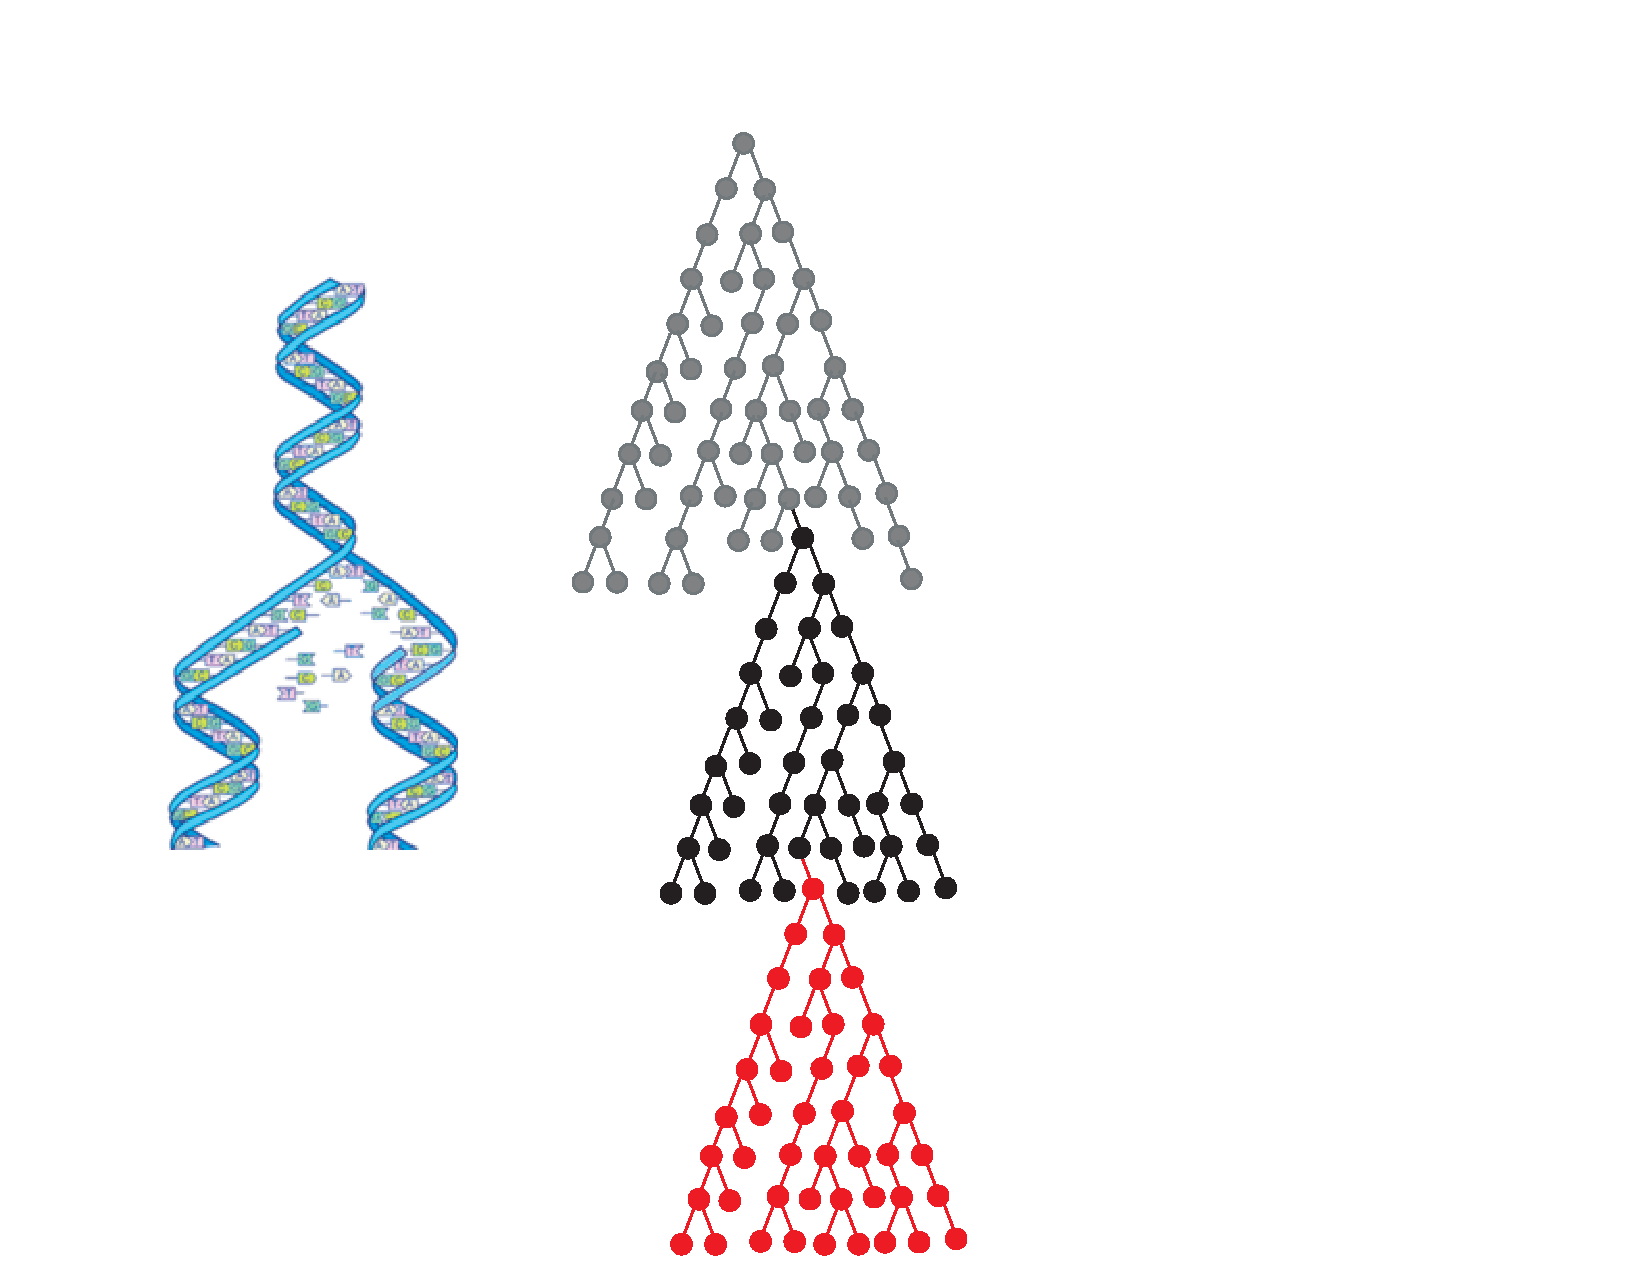
\includegraphics[scale=1.0]{../images/cellPhylogeny.pdf}}}
\end{picture}

\myNewSlide
\section*{Two types of genealogies}
\begin{picture}(0,0)(0,0)  \put(15,-45){\makebox(0,0)[l]{\includegraphics[scale=1.2]{../nonfreeimages/joe/toko_phylo.pdf}}}
\end{picture}

\myNewSlide
\section*{Genealogies within a population}
\unitlength=1mm
\begin{picture}(0,0)(0,0)  \put(15,-55){\makebox(0,0)[l]{\includegraphics[scale=1.2]{../nonfreeimages/joe/wright1.pdf}
}}
\put(65,5){Present}
\put(70,-125){Past}
\end{picture}

\myNewSlide
\section*{Genealogies within a population}
\unitlength=1mm
\begin{picture}(0,0)(0,0)  \put(15,-55){\makebox(0,0)[l]{\includegraphics[scale=1.2]{../nonfreeimages/joe/wright2.pdf}
}}
\put(65,5){Present}
\put(70,-125){Past}
\end{picture}

\myNewSlide
\section*{Genealogies within a population}
\unitlength=1mm
\begin{picture}(0,0)(0,0)  \put(15,-55){\makebox(0,0)[l]{\includegraphics[scale=1.2]{../nonfreeimages/joe/wright3.pdf}
}}
\put(65,5){Present}
\put(70,-125){Past}
\end{picture}

\myNewSlide
\section*{Genealogies within a population}
\unitlength=1mm
\begin{picture}(0,0)(0,0)  \put(15,-55){\makebox(0,0)[l]{\includegraphics[scale=1.2]{../nonfreeimages/joe/wright9.pdf}
}}
\put(65,5){Present}
\put(70,-125){Past}
\end{picture}

\myNewSlide
\section*{Genealogies within a population}
\unitlength=1mm
\begin{picture}(0,0)(0,0)  \put(15,-55){\makebox(0,0)[l]{\includegraphics[scale=1.2]{../nonfreeimages/joe/wright10.pdf}
}}
\put(65,5){Present}
\put(70,-125){Past}
\put(65,15){Present}
\put(70,-115){Past}
\put(-20,-135){Biparental inheritance would make the picture messier, but the genealogy}
\put(-10,-145){of the gene copies would still form a tree (if there is no recombination).}
\end{picture}

\myNewSlide
\section*{terminology: genealogical trees within population or species trees}
It is tempting to refer to the tips of these gene trees as alleles or haplotypes.
\begin{compactitem}
	\item allele -- an alternative form a gene. 
	\item haplotype -- a linked set of alleles
\end{compactitem}
But both of these terms require a differences in sequence.

The gene trees that we draw depict genealogical relationships -- regardless of whether or not nucleotide differences distinguish the ``gene copies'' at the tips of the tree.


\myNewSlide
\unitlength=1mm
\begin{picture}(0,0)(0,0)  \put(-55,-70){\makebox(0,0)[l]{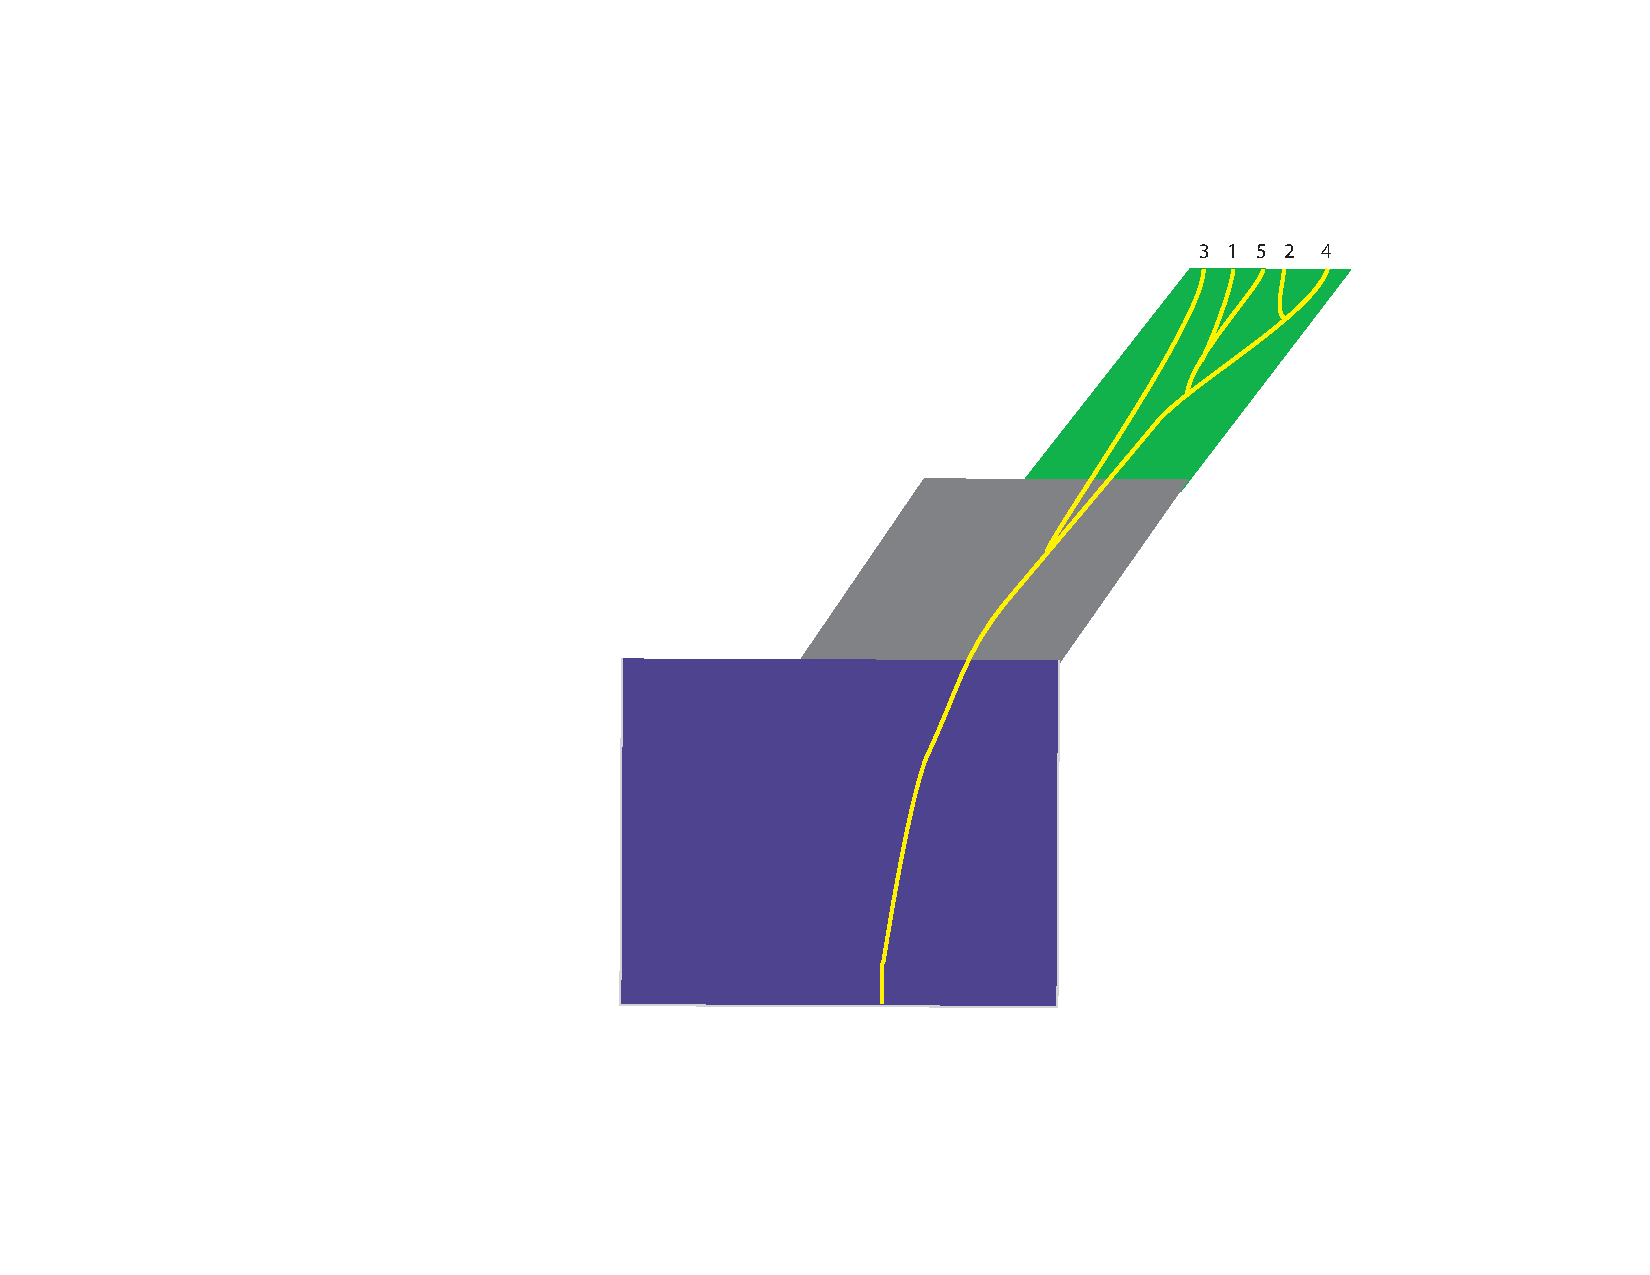
\includegraphics[scale=1.2]{../images/gene_tree_sp_tree_one_sp1.pdf}}}
\end{picture}

\myNewSlide
\unitlength=1mm
\begin{picture}(0,0)(0,0)  \put(-55,-70){\makebox(0,0)[l]{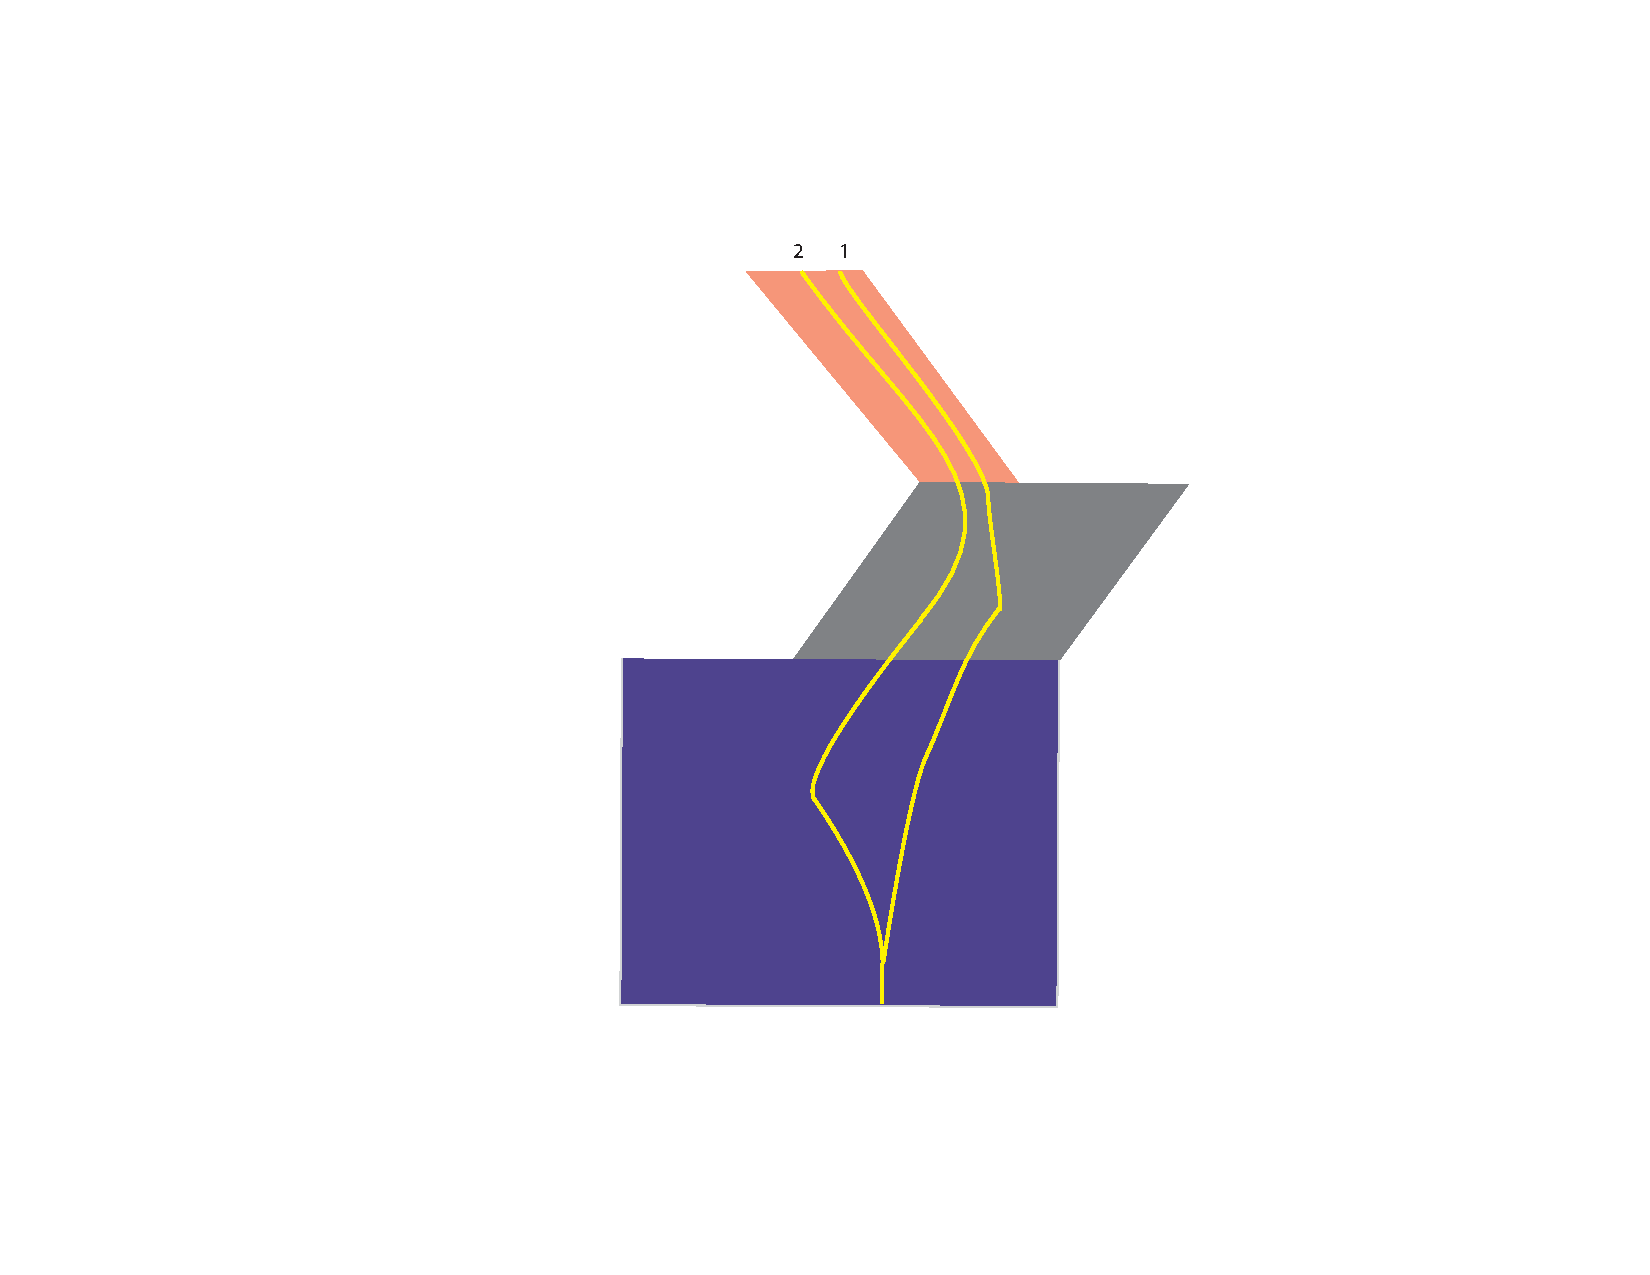
\includegraphics[scale=1.2]{../images/gene_tree_sp_tree_one_sp2.pdf}}}
\end{picture}

\myNewSlide

\section*{A ``gene tree'' within a species tree}
\unitlength=1mm
\begin{picture}(0,0)(0,0)  \put(-55,-70){\makebox(0,0)[l]{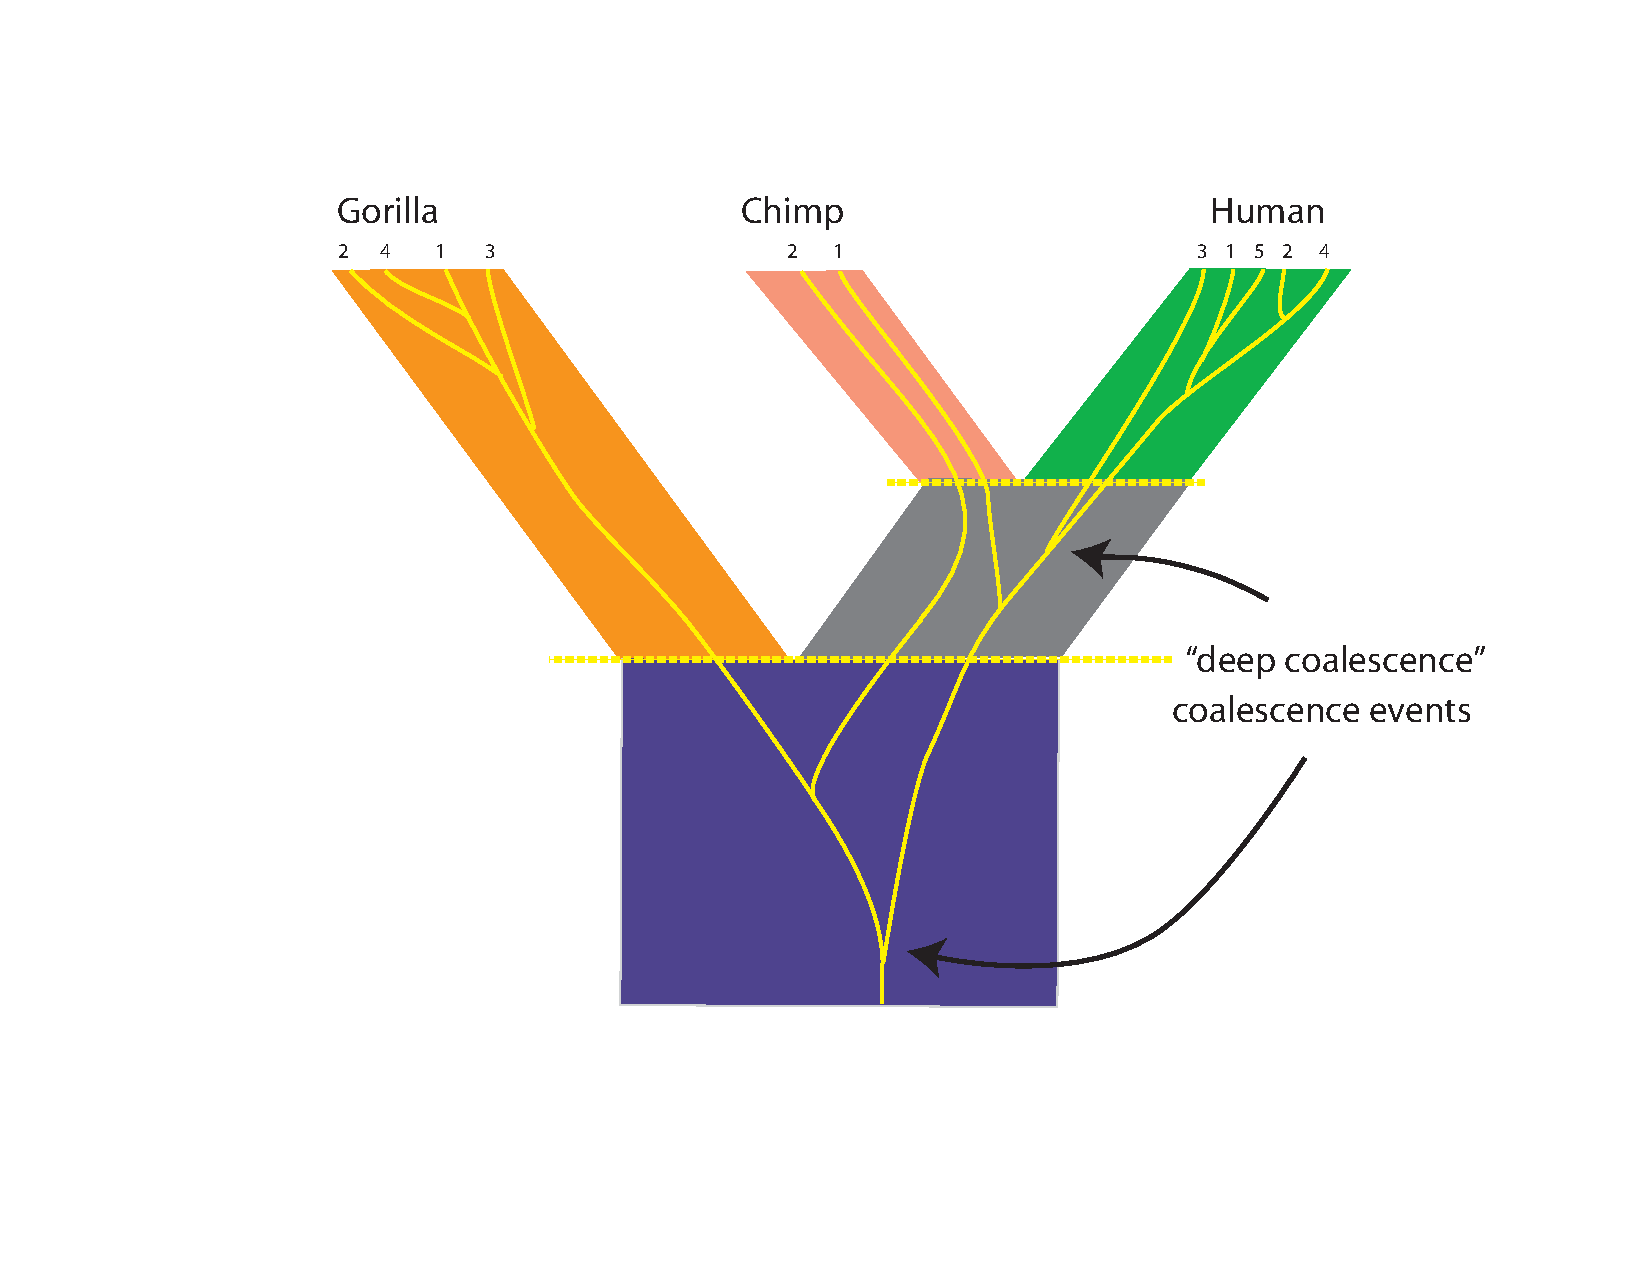
\includegraphics[scale=1.2]{../images/gene_tree_sp_tree.pdf}}}
\end{picture}

\myNewSlide
\section*{terminology: genealogical trees within population or species trees}
\begin{itemize}
	\item coalescence -- merging of the genealogy of multiple gene copies into their common ancestor.  ``Merging'' only makes sense when viewed {\em backwards in time}.
	\item ``deep coalescence'' or ``incomplete lineage sorting'' refer to the {\em failure} of gene copies to coalesce within the duration of the species -- the lineages coalesce in an ancestral species
\end{itemize}


\myNewSlide
\section*{terminology: genealogical trees within population or species trees}
\begin{itemize}
	\item coalescence -- merging of the genealogy of multiple gene copies into their common ancestor.  ``Merging'' only makes sense when viewed {\em backwards in time}.
	\item ``deep coalescence'' or ``incomplete lineage sorting'' refer to the {\em failure} of gene copies to coalesce within the duration of the species -- the lineages coalesce in an ancestral species
\end{itemize}


\myNewSlide
\section*{A ``gene family tree''}
\unitlength=1mm
\begin{picture}(0,0)(0,0)
  \put(-15,-60){\makebox(0,0)[l]{\includegraphics[scale=1.1]{../nonfreeimages/other/OpazoHS2008Fig1.pdf}}}
\put(170,-55){\small Opazo, Hoffmann and Storz}
\put(170,-63){\small``Genomic evidence for}
\put(170,-71){\small independent origins of $\beta$-like}
\put(170,-79){\small globin genes in monotremes }
\put(170,-88){\small and therian mammals''}
\put(170,-97){\small PNAS {\bf 105(5)} 2008}
\end{picture}


\myNewSlide
\unitlength=1mm
\begin{picture}(0,0)(0,0)
  \put(15,-60){\makebox(0,0)[l]{\includegraphics[scale=1.2]{../nonfreeimages/other/OpazoHS2008Fig4.pdf}}}
\put(-15,-150){\small Opazo, Hoffmann and Storz ``Genomic evidence for independent origins of $\beta$-like}
\put(-15,-158){\small globin genes in monotremes and therian mammals'' PNAS {\bf 105(5)} 2008}
\end{picture}

\myNewSlide
\section*{terminology: trees of gene families}
\begin{itemize}
	\item duplication -- the creation of a new copy of a gene within the same genome.
	\item homologous -- descended from a common ancestor.
	\item paralogous --  homologous, but resulting from a gene duplication in the common ancestor. 
	\item orthologous -- homologous, and resulting from a speciation event at the common ancestor.
\end{itemize}


\myNewSlide
Multiple contexts for tree estimation (again):
\begin{table}[htdp]
\begin{center}
\begin{tabular}{|p{5cm}|p{5cm}|p{11cm}|}
& {\bf The cause of splitting} & {\bf Important caveats} \\
\hline
``Gene tree'' & DNA replication & recombination is usually ignored \\
\hline
Species tree Phylogeny & speciation & recombination, hybridization, and deep coalescence cause conflict in the data we use to estimate phylogenies\\
\hline
Gene family tree & speciation or duplication & recombination (eg. domain swapping) is not tree-like \\
\hline
\end{tabular}
\end{center}
\label{default}
\end{table}%

\myNewSlide
\large 
Phylogeny with complete genome + ``phenome'' as colors:\\
\normalsize 
\begin{picture}(0,0)(20,0)
	\put(30,-80){\makebox(0,0)[l]{\includegraphics[scale=1.]{../images/InstantSpWithFixation.pdf}}}
	\put(-0,-110){This figure:}
	\put(0,-120){dramatically underestimates}
	\put(5,-130){ polymorphism}
	\put(0,-140){ignore geographic aspects}
	\put(5,-150){of speciation and character evolution}
\end{picture}


\myNewSlide
\large 
Extant species are just a thin slice of the phylogeny:\\
\begin{picture}(0,0)(20,0)
	\put(30,-80){\makebox(0,0)[l]{\includegraphics[scale=1.]{../images/InstantSpFinalSp.pdf}}}
\end{picture}

\myNewSlide
\large 
Our exemplar specimens are a subset of the current diversity:\\
\begin{picture}(0,0)(20,0)
	\put(30,-80){\makebox(0,0)[l]{\includegraphics[scale=1.]{../images/InstantSpData.pdf}}}
\end{picture}

\myNewSlide
\large 
The phylogenetic inference problem:\\
\begin{picture}(0,0)(20,0)
	\put(30,-120){\makebox(0,0)[l]{\includegraphics[scale=1.]{../images/InstantSpInferenceProblem.pdf}}}
\end{picture}

\myNewSlide
\begin{picture}(0,0)(0,0)
	\put(10,-60){\makebox(0,0)[l]{\includegraphics[scale=1.0]{../images/InstantSpWithFixationTS.pdf}}}
\end{picture}

\myNewSlide
\begin{picture}(0,0)(0,0)
	\put(10,-160){\makebox(0,0)[l]{\includegraphics[scale=1.0]{../images/InstantSpWithFixTSSimple.pdf}}}
\end{picture}

\myNewSlide
\begin{picture}(0,0)(0,0)
	\put(10,-100){\makebox(0,0)[l]{\includegraphics[scale=1.0]{../images/InstantSpWithFixTSSimpleInfer.pdf}}}
\end{picture}

\myNewSlide
\begin{picture}(0,0)(0,0)
	\put(10,-100){\makebox(0,0)[l]{\includegraphics[scale=1.0]{../images/InstantSpWithFixTSRejectInfer.pdf}}}
	\put(-20,-120){Multiple origins}
	\put(-20,-130){of the yellow state}
	\put(-20,-140){violates our assumption}
	\put(-20,-150){that the state codes in}
	 \put(-20,-160){our transformation scheme}
	 \put(-20,-170){represent homologous states}
\end{picture}

\myNewSlide
\begin{picture}(0,0)(0,0)
	\put(-95,-160){\makebox(0,0)[l]{\includegraphics[scale=2.0]{../images/InstantSpWithFixTSComplex.pdf}}}
\end{picture}


\myNewSlide
Character matrices:\\
\begin{table}[htdp]
\begin{center}
\begin{tabular}{|c|c|c|c|c|c|c|c|}
\hline
&  & \multicolumn{6}{c|}{Characters} \\
& & 1 & 2 & 3 & 4 & 5 & 6 \\
\hline
\multirow{3}{*}{Taxa} & {\em Homo sapiens} & 0.13 & A & A & rounded & 1 & 1610 - 1755 \\
 & {\em Pan paniscus} & 0.34 & A & G & flat & 2 & 0621 - 0843 \\
  & {\em Gorilla gorilla} & 0.46 & C & G & pointed & 1 & 795 - 1362\\
\hline
\end{tabular}
\end{center}
\label{default}
\end{table}
Characters (aka ``transformation series'') are the columns.\\
The values in the cells are character states (aka ``characters'').\\

\myNewSlide
\begin{table}[htdp]
\begin{center}
\begin{tabular}{|c|c|c|c|c|c|c|c|}
\hline
&  & \multicolumn{6}{c|}{Characters} \\
& & 1 & 2 & 3 & 4 & 5 & 6 \\
\hline
\multirow{3}{*}{Taxa} & {\em Homo sapiens} & 0.13 & A & A & rounded & 1 & 1610 - 1755 \\
 & {\em Pan paniscus} & 0.34 & A & G & flat & 2 & 0621 - 0843 \\
  & {\em Gorilla gorilla} & 0.46 & C & G & pointed & 1 & 795 - 1362\\
\hline
\end{tabular}
\end{center}
\label{default}
\end{table}
Character coding:
\begin{table}[htdp]
\begin{center}
\begin{tabular}{|c|c|c|c|c|c|c|c|}
\hline
&  & \multicolumn{6}{c|}{Characters} \\
& & 1 & 2 & 3 & 4 & 5 & 6 \\
\hline
\multirow{3}{*}{Taxa} & {\em Homo sapiens} & 0 & A & A & 0 & 1 & 4 \\
 & {\em Pan paniscus} & 2 & A & G & 1 & 2 & 0,1 \\
  & {\em Gorilla gorilla} & 3 & C & G & 2 & 1 & 1,2\\
\hline
\end{tabular}
\end{center}
\label{default}
\end{table}

\myNewSlide
\Large
The meaning of homology ({\bf very roughly}):
\begin{compactenum}
	\item comparable (when applied to characters) 
	\item identical by descent (when applied to character states) 
\end{compactenum}

Ideally, each possible character state would arise once in the 
entire history of life on earth.

\myNewSlide
\large
Instances of the filled character state are homologous\\
Instances of the hollow character state are homologous\\
\begin{picture}(0,0)(20,0)  \put(30,-80){\makebox(0,0)[l]{\includegraphics[scale=1.]{../nonfreeimages/pol/monophyletic.pdf}}}
\end{picture}

\myNewSlide
Instances of the filled character state are homologous\\
Instances of the hollow character state are NOT homologous\\
\begin{picture}(0,0)(0,0)
	\put(30,-80){\makebox(0,0)[l]{\includegraphics[scale=1.0]{../images/paraphyletic.pdf}}}
\end{picture}

\myNewSlide
Instances of the filled character state are NOT homologous\\
Instances of the hollow character state are homologous\\
\begin{picture}(0,0)(0,0)
	\put(30,-80){\makebox(0,0)[l]{\includegraphics[scale=1.0]{../images/polyphyletic.pdf}}}
\end{picture}



\myNewSlide
\section*{Inference}
``deriving a conclusion based solely on what one already knows''\footnote{definition from Wikipedia, so it must be correct!}
\begin{compactitem}
	\item logical
	\item statistical
\end{compactitem}



\myNewSlide
\begin{picture}(0,0)(20,20)
	\put(35,-153){\makebox(0,0)[l]{\includegraphics[scale=1.5]{../images/tree_to_data0.pdf}}}
\end{picture}

\myNewSlide
\begin{picture}(0,0)(20,20)
	\put(35,-153){\makebox(0,0)[l]{\includegraphics[scale=1.5]{../images/tree_to_data0_5.pdf}}}
\end{picture}

\myNewSlide
\begin{picture}(0,0)(20,20)
	\put(35,-173){\makebox(0,0)[l]{\includegraphics[scale=1.5]{../images/tree_to_data.pdf}}}
\end{picture}


\myNewSlide
\begin{picture}(0,0)(20,20)
	\put(35,-173){\makebox(0,0)[l]{\includegraphics[scale=1.5]{../images/tree_to_data2.pdf}}}
\end{picture}


\myNewSlide
\begin{picture}(0,0)(20,20)
	\put(35,-153){\makebox(0,0)[l]{\includegraphics[scale=1.5]{../images/tree_to_data3.pdf}}}
\end{picture}


\myNewSlide
\begin{picture}(0,0)(20,20)
	\put(35,-153){\makebox(0,0)[l]{\includegraphics[scale=1.5]{../images/tree_to_data4.pdf}}}
\end{picture}



\myNewSlide
\section*{Logical Inference}
Deductive reasoning:
\begin{compactenum}
	\item start from premises
	\item apply proper rules
	\item arrive at statements that were not obviously contained in the premises.
\end{compactenum}
If the rules are valid (logically sound) and the premises are true, then the conclusions are {\em guaranteed} to be true.

\myNewSlide
\section*{Deductive reasoning}
\begin{verbatim}
All men are mortal.
Socrates is a man.
-------------------
Therefore Socrates is mortal. 
\end{verbatim}
\vskip 3cm
Can we infer phylogenies from character data using deductive reasoning?

\myNewSlide
\section*{Logical approach to phylogenetics}
Premise: The following character matrix is correctly coded (character states are 
homologous in the strict sense):\\

\begin{table}[htdp]
\begin{center}
\begin{tabular}{l|c}
 & {1} \\
\hline
{taxon A} & Z\\
{taxon B}  & Y \\
{taxon C}  & Y \\
\end{tabular}
\end{center}
\label{default}
\end{table}

Is there a valid set of rules that will generate the tree
as a conclusion?

\myNewSlide
\section*{Logical approach to phylogenetics (cont)}
Rule: Two taxa that share a character state must be more closely
related to each other than either is to a taxon that displays
a different state.

Is this a valid rule?

\myNewSlide
\section*{Invalid rule}
Here is an example in which we are confident that the homology statements
are correct, but our rule implies two conflicting trees:
\begin{table}[htdp]
\begin{center}
\begin{tabular}{l|c|c}
 & {\begin{sideways}\parbox{15mm}{placenta}\end{sideways}} & {\begin{sideways}\parbox{35mm}{vertebra}\end{sideways}}\\
\hline
{\em Homo sapiens} & Z & A \\
{\em Rana catesbiana}  & Y & A \\
{\em Drosophila melanogaster}  & Y & B \\

\end{tabular}
\end{center}
\label{default}
\end{table}

\myNewSlide
\section*{Hennigian logical analysis}
The German entomologist Willi Hennig (in addition to 
providing strong arguments for phylogenetic classifications)
clarified the logic of phylogenetic inference.

Hennig's correction to our rule: Two taxa that share a 
{\bf derived} character state must be more closely
related to each other than either is to a taxon that 
displays the {\bf primitive} state.



\myNewSlide
\section*{Hennig's logic is valid}
Here we will use 0 for the primitive state, and 1 for the derived state.
\begin{table}[htdp]
\begin{center}
\begin{tabular}{l|c|c}
 & {\begin{sideways}\parbox{15mm}{placenta}\end{sideways}} & {\begin{sideways}\parbox{35mm}{vertebra}\end{sideways}}\\
\hline
{\em Homo sapiens} & 1 & 1 \\
{\em Rana catesbiana}  & 0 & 1 \\
{\em Drosophila melanogaster}  & 0 & 0 \\
\end{tabular}
\end{center}
\label{default}
\end{table}
Now the character ``placenta'' does not provide a grouping, but ``vertebra''
groups human and frog as sister taxa.

\myNewSlide
\section*{Hennigian terminology}
prefixes:
\begin{compactitem}
	\item ``apo'' - refers to the new or derived state
	\item ``plesio'' - refers to the primitive state
    \item ``syn'' or ``sym'' - used to indicate shared between taxa
    \item ``aut'' - used to indicate a state being unique to one taxon
\end{compactitem}

\myNewSlide
\section*{Hennigian rules}
\begin{compactitem}
	\item synapomorphy - shared, derived states. Used to diagnose monophyletic groups.
	\item symplesiomorphy - shared, primitive states. Diagnose icky, unwanted paraphyletic groups.
	 \item autapomorphy -- a unique derived state. {\bf No} evidence of phylogenetic relationships.
	 \item constant characters -- columns in a matrix with no variability between taxa. {\bf No} evidence of phylogenetic relationships.
\end{compactitem}

\myNewSlide
\begin{picture}(0,0)(0,0)
	\put(-10,-60){\makebox(0,0)[l]{\includegraphics[scale=1.2]{../images/ppmphyletic.pdf}}}
\end{picture}


\myNewSlide
\section*{Hennigian inference}
When we create a character matrix for Hennig's system, it is crucial that:
\begin{compactitem}
	\item traits assigned the same state represent homologous states (trace back to the MRCA)
	\item we correctly identify the directionality of the transformations (which state is plesiomorphic and which is apomorphic).
	The process of identifying the direction of change is called polarization.
\end{compactitem}

Polarization could be done based on developmental considerations, paleontological evidence, or biogeographic considerations, but the most common technique is outgroup polarization.



\myNewSlide
\begin{table}[htdp]
\begin{center}
\label{coloredPerfect}
\begin{tabular}{|c|c|c|c|c|c|c|c|c|c|c|}
\hline 
 & \multicolumn{10}{c|}{Character \#} \\ 
Taxon &\color{blue} 1 & \color{blue} 2 & \color{blue} 3 & \color{blue} 4 & \color{blue} 5 & \color{green} 6 & \color{green} 7 & \color{green} 8 & \color{green} 9 & \color{red} 10  \\ 
\hline 
A &    \color{blue} 0 & \color{blue} 0 & \color{blue} 0 & \color{blue} 0 & \color{blue} 0 & \color{green} 0 & \color{green} 0 & \color{green} 0 & \color{green} 0 & \color{red} 0 \\
B &    \color{blue} 1 & \color{blue} 0 & \color{blue} 0 & \color{blue} 0 & \color{blue} 0 & \color{green} 1 & \color{green} 1 & \color{green} 1 & \color{green} 1 & \color{red} 1 \\
C &    \color{blue} 0 & \color{blue} 1 & \color{blue} 1 & \color{blue} 1 & \color{blue} 0 & \color{green} 1 & \color{green} 1 & \color{green} 1 & \color{green} 1 & \color{red} 1 \\
D &    \color{blue} 0 & \color{blue} 0 & \color{blue} 0 & \color{blue} 0 & \color{blue} 1 & \color{green} 1 & \color{green} 1 & \color{green} 1 & \color{green} 1 & \color{red} 0 \\
\hline 
\end{tabular}
\end{center}
\end{table}

\myNewSlide
\begin{center}
\begin{picture}(-90,0)(20,20)
	\thicklines
	\put(-26,17){B} 
	\put(14,-53){C} 
	\put(-46,-93){D}
	\put(-50,20){\line(1,0){20}} 
	\put(-50,-50){\line(1,0){60}} 
	\put(-50,-50){\line(0,1){70}} 
	\put(-70,-10){\line(1,0){20}} 
	\put(-70,-90){\line(1,0){20}} 
	\put(-70,-90){\line(0,1){80}} 
	\put(-150,-50){\line(1,0){80}}
	\put(-150,-120){\line(1,0){10}} 
	\put(-150,-120){\line(0,1){70}} 
	\put(-136,-123){A} 
	\put(50,7){B C} 
	\put(-40,17){\color{blue} \line(0,1){6}}
	\put(-42,7){\color{blue}1}
	\put(-33,-53){\color{blue} \line(0,1){6}}
	\put(-24,-53){\color{blue} \line(0,1){6}}
	\put(-15,-53){\color{blue} \line(0,1){6}}
	\put(-35,-63){\color{blue}2 3 4}
	\put(-60,-93){\color{blue} \line(0,1){6}}
	\put(-62,-103){\color{blue}5}
	\put(-60,-13){\color{red} \line(0,1){6}}
	\put(-66,-23){\color{red}10}
	\put(-123,-53){\color{green} \line(0,1){6}}
	\put(-113,-53){\color{green} \line(0,1){6}}
	\put(-104,-53){\color{green} \line(0,1){6}}
	\put(-95,-53){\color{green} \line(0,1){6}}
	\put(-125,-63){\color{green}6 7 8 9}
	\put(55,10){\oval(30,20)} 
	\put(55,-10){D} 
	\put(65,5){\oval(60,40)} 
	\put(55,-27){A}
\end{picture}
\end{center}

\myNewSlide
Interestingly, without polarization Hennig's method
can infer unrooted trees.
We can get the tree topology, but be unable to tell 
paraphyletic from monophyletic groups.

The outgroup method amounts to inferring an unrooted
tree and then rooting the tree on the branch that
leads to an outgroup.

\myNewSlide
\begin{center}
\begin{picture}(-90,0)(20,20)
	\thicklines
	\put(-26,17){B} 
	\put(14,-53){C} 
	\put(-99,17){D}
	\put(-50,20){\line(1,0){20}} 
	\put(-50,-50){\line(1,0){60}} 
	\put(-50,-50){\line(0,1){70}} 
	\put(-70,-10){\line(1,0){20}} 
	\put(-90,20){\line(1,0){20}} 
	\put(-70,-50){\line(0,1){70}} 
	\put(-140,-50){\line(1,0){70}}
	\put(-150,-55){A} 
	\put(50,7){B}
	\put(50,-20){A}
 	\put(35,-5){\color{red}\line(1,0){70}} 
	\put(80,7){C} 
	 \put(80,-20){D} 
	\put(-40,17){\color{blue} \line(0,1){6}}
	\put(-42,7){\color{blue}1}
	\put(-33,-53){\color{blue} \line(0,1){6}}
	\put(-24,-53){\color{blue} \line(0,1){6}}
	\put(-15,-53){\color{blue} \line(0,1){6}}
	\put(-35,-63){\color{blue}2 3 4}
	\put(-80,17){\color{blue} \line(0,1){6}}
	\put(-82,7){\color{blue}5}
	\put(-60,-13){\color{red} \line(0,1){6}}
	\put(-66,-23){\color{red}10}
	\put(-123,-53){\color{green} \line(0,1){6}}
	\put(-113,-53){\color{green} \line(0,1){6}}
	\put(-104,-53){\color{green} \line(0,1){6}}
	\put(-95,-53){\color{green} \line(0,1){6}}
	\put(-125,-63){\color{green}6 7 8 9}
\end{picture}
\end{center}


\myNewSlide
\section*{Inadequacy of logic}
Unfortunately, though Hennigian logic is valid we quickly find that we
do not have a reliable method of generating accurate homology statements.

The logic is valid, but we don't know that the premises are true.  

In fact, we almost always find that it is impossible for all of our premises to be true.

\myNewSlide
\section*{Character conflict}
\begin{table}[htdp]
\begin{center}
\begin{tabular}{l|l}
 &  \\
\hline
{\em Homo sapiens} & {\tt A{\color{red} G}TTCAAG{\color{green} T}} \\
{\em Rana catesbiana}  & {\tt A{\color{red} A}TTCAAG{\color{green} T}} \\
{\em Drosophila melanogaster}  & {\tt A{\color{red} G}TTCAAG{\color{green} C}} \\
{\em C. elegans}  & {\tt A{\color{red} A}TTCAAG{\color{green} C}} \\
\end{tabular}
\end{center}
\label{default}
\end{table}
The red character implies that either ({\em Homo + Drosophila}) is a group (if G is derived) and/or
({\em Rana + C. elegans}) is a group.\\
The green character implies that either ({\em Homo + Rana}) is a group (if T is derived) and/or
({\em Drosophila + C. elegans}) is a group.\\
The green and red character cannot both be correct.


\myNewSlide
\begin{table}[htdp]
\begin{center}
\label{coloredHomoplasy}
\begin{tabular}{|c|c|c|c|c|c|c|c|c|c|c|c|c|c|}
\hline 
 & \multicolumn{12}{c|}{Character \#} \\ 
Taxon &\color{blue} 1 & \color{blue} 2 & \color{blue} 3 & \color{blue} 4 & \color{blue} 5 & \color{green} 6 & \color{green} 7 & \color{green} 8 & \color{green} 9 & \color{red} 10 & \color{red} 11 &  \color{red} 12   \\ 
\hline 
A & \color{blue} 0 & \color{blue} 0 & \color{blue} 0 & \color{blue} 0 & \color{blue} 0 & \color{green} 0 & \color{green} 0 & \color{green} 0 & \color{green} 0 & \color{red} 0 & \color{red} 0 & \color{red} 0  \\
B & \color{blue} 1 & \color{blue} 0 & \color{blue} 0 & \color{blue} 0 & \color{blue} 0 & \color{green} 1 & \color{green} 1 & \color{green} 1 & \color{green} 1 & \color{red} 1 & \color{red} 1 & \color{red} 1 \\
C &    \color{blue} 0 & \color{blue} 1 & \color{blue} 1 & \color{blue} 1 & \color{blue} 0 & \color{green} 1 & \color{green} 1 & \color{green} 1 & \color{green} 1 & \color{red} 1 & \color{red} 1 & \color{red} 0\\
D &    \color{blue} 0 & \color{blue} 0 & \color{blue} 0 & \color{blue} 0 & \color{blue} 1 & \color{green} 1 & \color{green} 1 & \color{green} 1 & \color{green} 1 & \color{red} 0 & \color{red} 0 & \color{red} 1\\
\hline 
\end{tabular}
\end{center}
\end{table}



\myNewSlide
\begin{figure}
\begin{center}
\label{mpnesting}
\begin{picture}(0,0)(20,20)
	\thicklines
	\put(15,-35){C} 
	\put(-45,-35){B} 
	\put(-45,-75){D} 
	\put(19,-32){{\color{blue}\oval(40,40)}} 
	\put(19,-32){{\color{blue}\oval(30,30)}} 
	\put(19,-32){{\color{blue}\oval(20,20)}} 
	\put(-41,-72){{\color{blue}\oval(20,20)}} 
	\put(-41,-32){{\color{blue}\oval(20,20)}} 
	\put(-40,-52){{\color{red}\oval(30,70)}} 
	\put(-10,-32){{\color{red}\oval(120,45)}} 
	\put(-10,-32){{\color{red}\oval(125,52)}} 
	\put(15,-47){{\color{green}\oval(180,95)}} 
	\put(15,-47){{\color{green}\oval(185,102)}} 
	\put(15,-47){{\color{green}\oval(190,109)}} 
	\put(15,-47){{\color{green}\oval(195,116)}} 
	\put(135,-30){A} 
\end{picture}
\end{center}
\vskip 4.1cm
\end{figure}


\myNewSlide
\bibliography{../phylo848}

\end{document}